% Format teze zasnovan je na paketu memoir
% http://tug.ctan.org/macros/latex/contrib/memoir/memman.pdf ili
% http://texdoc.net/texmf-dist/doc/latex/memoir/memman.pdf
% 
% Prilikom zadavanja klase memoir, navedenim opcijama se podešava 
% veličina slova (12pt) i jednostrano štampanje (oneside).
% Ove parametre možete menjati samo ako pravite nezvanične verzije
% mastera za privatnu upotrebu (na primer, u b5 varijanti ima smisla 
% smanjiti 
\documentclass[12pt,oneside]{memoir} 
% Paket koji definiše sve specifičnosti master rada Matematičkog fakulteta
\usepackage[latinica]{matfmaster} 
\usepackage{pgf-umlcd}


\usepackage{listings}
\usepackage{float}
\floatstyle{plaintop}
\restylefloat{table}

\newtheorem{primer}{Primer}[section]


\lstdefinestyle{customc}{
  belowcaptionskip=1\baselineskip,
  breaklines=true,
  frame=L,
  xleftmargin=\parindent,
  language=C++,
  showstringspaces=false,
  basicstyle=\footnotesize\ttfamily,
  keywordstyle=\bfseries\color{green!40!black},
  commentstyle=\itshape\color{purple!40!black},
  identifierstyle=\color{blue},
  stringstyle=\color{orange},
  numbers=left,
  numberstyle=\tiny,
}

\lstdefinestyle{customasm}{
  belowcaptionskip=1\baselineskip,
  frame=L,
  xleftmargin=\parindent,
  language=[x86masm]Assembler,
  basicstyle=\footnotesize\ttfamily,
  commentstyle=\itshape\color{purple!40!black},
}


\lstdefinestyle{BashInputStyle}{
  language=bash,
  belowcaptionskip=1\baselineskip,
  basicstyle=\small\sffamily,
  numbers=left,
  numberstyle=\tiny,
  numbersep=3pt,
  frame=tb,
  columns=fullflexible,
  backgroundcolor=\color{yellow!20},
  linewidth=0.9\linewidth,
  xleftmargin=0.1\linewidth,
}

\lstdefinestyle{custombash}{
  belowcaptionskip=1\baselineskip,
  frame=L,
  xleftmargin=\parindent,
  language=[x86masm]Assembler,
  basicstyle=\footnotesize\ttfamily,
  commentstyle=\itshape\color{purple!40!black},
  captionpos=t,
  % backgroundcolor=\color{yellow!20},
  numbers=left,
  numberstyle=\tiny,
}

% \usepackage[serbian]{babel}%
% Podrazumevano pismo je ćirilica.
%   Ako koristite pdflatex, a ne xetex, sav latinički tekst na srpskom jeziku
%   treba biti okružen sa \lat{...} ili \begin{latinica}...\end{latinica}.
%
% Opicija [latinica]:
%   ako želite da pišete latiniciom, dodajte opciju "latinica" tj.
%   prethodni paket uključite pomoću: \usepackage[latinica]{matfmaster}.
%   Ako koristite pdflatex, a ne xetex, sav ćirilički tekst treba biti
%   okružen sa \cir{...} ili \begin{cirilica}...\end{cirilica}.
%
% Opcija [biblatex]:
%   ako želite da koristite reference na više jezika i umesto paketa
%   bibtex da koristite BibLaTeX/Biber, dodajte opciju "biblatex" tj.
%   prethodni paket uključite pomoću: \usepackage[biblatex]{matfmaster}
%
% Opcija [b5paper]:
%   ako želite da napravite verziju teze u manjem (b5) formatu, navedite
%   opciju "b5paper", tj. prethodni paket uključite pomoću: 
%   \usepackage[b5paper]{matfmaster}. Tada ima smisla razmisliti o promeni
%   veličine slova (izmenom opcije 12pt na 11pt u \documentclass{memoir}).
%
% Naravno, opcije je moguće kombinovati.
% Npr. \usepackage[b5paper,biblatex]{matfmaster}

% Pomoćni paket koji generiše nasumičan tekst u kojem se javljaju sva slova
% azbuke (nema potrebe koristiti ovo u pravim disertacijama)
% \usepackage[latinica]{pangrami}

% Datoteka sa literaturom u BibTex tj. BibLaTeX/Biber formatu
\bib{MasterRadOgnjenPlavsic}

% Ime kandidata na srpskom jeziku (u odabranom pismu)
\autor{Ognjen Ž. Plavšić}
% Naslov teze na srpskom jeziku (u odabranom pismu)
\naslov{Alat za stati\v{c}ku analizu i predlaganje izmena u C++ kodu}
% Godina u kojoj je teza predana komisiji
\godina{2022}
% Ime i afilijacija mentora (u odabranom pismu)
\mentor{dr Milena \textsc{Vujošević Janičić}, vanredni profesor\\ Univerzitet u Beogradu, Matematički fakultet}
% Ime i afilijacija prvog člana komisije (u odabranom pismu)
\komisijaA{dr Filip \textsc{Marić}, vanredni profesor\\ Univerzitet u Beogradu, Matematički fakultet}
% Ime i afilijacija drugog člana komisije (u odabranom pismu)
\komisijaB{dr Jelena \textsc{Graovac}, docent\\ Univerzitet u Beogradu, Matematički fakultet}
% Ime i afilijacija trećeg člana komisije (opciono)
% \komisijaC{}
% Ime i afilijacija četvrtog člana komisije (opciono)
% \komisijaD{}
% Datum odbrane (odkomentarisati narednu liniju i upisati datum odbrane ako je poznat)
% \datumodbrane{}

% Apstrakt na srpskom jeziku (u odabranom pismu)
\apstr{%
Standardi za pravilno pisanje C++ koda sve su zastupljeniji u industrijama koje razvijaju sisteme sa ugrađenim ra\v{c}unarom (eng.~\textit{embedded systems}) i druge sisteme
sa kriti\v{c}nom bezbedno\v{s}\'{c}u. Standard \textsc{autosar} C++14 jedan je od vode\'{c}ih standarda ovog tipa. Primarno se koristi u automobilskoj industriji, odnosno za
razvoj softvera za automobile. \v{S}iroka upotreba ovih standarda izrodila je potrebu za alatima za stati\v{c}ku analizu koji bi automatizovali proces provere da li je k\^{o}d napisan u skladu sa standardom. Kompilatorska infrastruktura LLVM pru\v{z}a podr\v{s}ku za jednostavno razvijanje kvalitetnih alata ovog tipa. Cilj ovog rada je implementacija alata za stati\v{c}ku analizu \textit{AutoFix} koji proverava da li je k\^{o}d napisan u skladu sa podskupom pravila koja se odnose na deklaracije u okviru standarda \textsc{autosar} C++14. Alat ispisuje upozorenja za delove koda koji nisu u skladu sa nekim od pravila i predla\v{z}e izmene tog koda. 
}
\usepackage{tcolorbox}
% Ključne reči na srpskom jeziku (u odabranom pismu)
\kljucnereci{verifikacija softvera, stati\v{c}ka analiza programa, programski jezik C++, standardi kodiranja, \textsc{autosar}, kompilatori, LLVM,  Clang}

\begin{document}
% ==============================================================================
% Uvodni deo teze
\frontmatter
% ==============================================================================
% Naslovna strana
\naslovna
% Strana sa podacima o mentoru i članovima komisije
\komisija
% Strana sa posvetom (u odabranom pismu)
\posveta{Porodici}
% Strana sa podacima o disertaciji na srpskom jeziku
\apstrakt
% Sadržaj teze
\tableofcontents*

% ==============================================================================
% Glavni deo teze
\mainmatter
% ==============================================================================

% ------------------------------------------------------------------------------
\chapter{Uvod}
% ------------------------------------------------------------------------------

Softver je neizostavni deo modernog sveta. U zavisnosti od primene softvera i konteksta u kome se koristi, kvalitet softvera mo\v{z}e da igra
manju ili ve\'{c}u ulogu. Na primer, gre\v{s}ke u video igri ima\'{c}e za posledicu samo nezadovoljstvo korisnika, dok gre\v{s}ke u softveru
za kontrolisanje ko\v{c}nica automobila mogu imati fatalne posledice. Iz ovog razloga određene industrije ula\v{z}u dodatni napor kako bi se uverile u kvalitet softvera
i kako bi smanjili mogu\'{c}nost pojave gre\v{s}ke. \par
Na\v{c}in da se smanji mogu\'{c}nost pojave gre\v{s}ke u kodu jeste definisanje strogog pravila kodiranja u izabranom programskom jeziku. Jedan takav standard za programski jezik C++14 (jezik C++ iz verzije standarda za 2014. godinu) predstavlja standard kodiranja \textsc{autosar} C++14. Ovaj standard primarno se primenjuje u automobilskoj industriji. S obzirom da industrije koje primenjuju ovaj standard \v{c}esto koriste jako kompleksne softvere, potrebno je automatizovati proces provere da li je k\^{o}d napisan u skladu sa standardom. U ovu svrhu koriste se alati za stati\v{c}ku analizu koda. \par Alati za stati\v{c}ku analizu proveravaju ispravnost programa bez njegovog izvr\v{s}avanja. Ovakvi alati se mogu implementirati na vi\v{s}e na\v{c}ina. Jednostavniji alati koriste informacije dobijene tokom kompilacije programa da utvrde da li k\^{o}d sadr\v{z}i gre\v{s}ku. Napredniji alati za stati\v{c}ku analizu vr\v{s}e i simboli\v{c}ko izvr\v{s}avanje programa, odnosno koriste razli\v{c}ite tehnike kojima simuliraju izvr\v{s}avanje programa, bez njegovog pokretanja \cite{Etran, AutoCheck}. \par
Kompilatorska infrastruktura LLVM omogu\'{c}ava izradu alata za stati\v{c}ku analizu. Ova infrastruktura sadr\v{z}i niz biblioteka koje omogu\'{c}avaju analizu informacija dobijenih tokom kompilacije, ali sadr\v{z}i i biblioteke koje omogu\'{c}avaju izradu samostalnih alata. Cilj ovog rada je implementacija alata za stati\v{c}ku analizu
\textit{AutoFix}. \textit{AutoFix} proverava da li je k\^{o}d napisan u skladu sa podskupom pravila iz standarda \textsc{autosar} C++14 koja se odnose na deklaracije u programskom jeziku C++14. Ukoliko k\^{o}d nije napisan u skladu sa nekim od tih pravila, alat prijavljuje upozorenje zajedno sa predlogom za ispravljanje koda. 

U glavi \ref{chp:autosar} opisan je programski jezik C++ i standard kodiranja \textsc{autosar} C++14. Opisana je klasifikacija pravila u okviru standarda i navedeni su primeri pravila koja pripadaju svakoj od grupa u okviru klasifikacije. U glavi \ref{chp:llvm} opisani su delovi kompilatorske strukture LLVM koji su kori\v{s}\'{c}eni za izradu alata \textit{AutoFix}. U glavi 4 opisana je implementacija alata \textit{AutoFix} i na\v{c}in upotrebe alata. Takođe, opisano je i svako od pravila iz standarda \textsc{autosar} C++14 koje alat podr\v{z}ava. U zaklju\v{c}ku iznet je osvrt na ceo rad i predlo\v{z}en je dalji tok razvoja alata \textit{AutoFix}.
\chapter{Standard kodiranja \textsc{AUTOSAR} C++14}
\label{chp:autosar}

\textit{AUTomotive Open System ARchitecture (\textsc{AUTOSAR})} je međunarodna organizacija proizvođača vozila, dobavljača, pružaoca usluga i kompanija iz automobilske industrije i industrija elektronike, poluprovodnika i softvera \cite{autosarWebsite}. 
Cilj organizacije je da stvori i uspostavi otvorenu i standardizovanu softversku arhitekturu za automobilske elektronske upravljačke jedinice (\textit{eng.~Electronic Control Units, skra\'{c}eno ЕCU}).
Radi ostvarenja pomenutih ciljeva \textsc{autosar} definiše, između ostalog, pravila kodiranja u programskom jeziku C++14 za sisteme sa kriti\v{c}nom bezbedno\v{s}\'{c}u. Glavni sektor primene standarda kodiranja \textsc{autosar} C++14 je automobilska industrija, međutim ovaj standard može biti primenjen
i na druge aplikacije za sisteme sa ugrađenim računarom. Ovaj standard predstavlja nadogradnju standarda MISRA C++:2008 \cite{AutosarGuidelines}.

\section{Programski jezik C++}

\textbf{C++} je programski jezik op\v{s}te namene. Kreirao ga je danski softverski in\v{z}enjer Bjarne Stroustrup kao ekstenziju programskog jezika C. U trenutku kreiranja, osnovno pro\v{s}irenje u odnosu na programski jezik C bile su klase. C++ pripada grupi objektno orijentisanih jezika. 

\subsection{Dizajn programskog jezika C++}

Programski jezik C++ zadr\v{z}ava osnovne ideje i koncepte jezika C. Takođe, jezik pru\v{z}a sintaksu koja omogu\'{c}ava direktan i koncizan pristup problemu koji re\v{s}ava.
U svrhu toga, C++ pru\v{z}a:
\begin{itemize}
  \item {Direktna preslikavanja ugrađenih operacija i tipova na hardver kako bi obezbedio efikasno kori\v{s}\'{c}enje memorije i efikasne operacije niskog nivoa (eng.~\textit{low-level operations}).}
  \item {Priu\v{s}tive (u smislu ra\v{c}unarskih resursa) i fleksibilne mehanizme apstrakcija za podr\v{s}ku korisni\v{c}ki definisanih tipova koji se mogu koristiti sa istom sintaksom, u istom obimu i sa istim performansama kao ugrađeni tipovi.}
\end{itemize}

Dizajn jezika C++ je fokusiran na tehnike programiranja koje se bave osnovnim pojmovima ra\v{c}unarstva kao \v{s}to su memorija, mutabilnost, apstrakcija, upravljanje ra\v{c}unarskim resursima, izra\v{z}avanje algoritama, rukovanje gre\v{s}kama i modularnost. Jezik je dizajniran sa ciljem da \v{s}to vi\v{s}e olak\v{s}a sistemsko programiranje, odnosno pisanje programa koji direktno koriste hardverske resurse i kod kojih su ovi resursi u velikoj meri ograni\v{c}eni \cite{TheC++ProgrammingLanguage}.


\subsection{Standard C++14}

Programski jezik C++ je standardizovan. U okviru međunarodne organizacije za standardizaciju (eng.~\textit{International Standard Organization}, skra\'{c}eno ISO), standard za programski jezik C++ propisuje radna grupa poznata kao JTC1/SC22/W\-G21 \cite{ISOWebsite}. Do sada je objavljeno \v{s}est revizija C++ standarda i trenutno se radi na reviziji C++23. 
\indent

Standard C++14 predstavlja pro\v{s}irenje standarda C++11 uglavnom manjim pobolj\v{s}anjima i ispravljanjem gre\v{s}aka iz standarda C++11. Standard C++11 sa druge strane uveo je velike izmene u odnosu na prethodnu reviziju standarda, C++03. \par
Standardi C++11/14 uveli su ve\'{c}inu fundamentalnih koncepta onog \v{s}to se danas smatra modernim jezikom C++. Ovde spadaju desne reference, "move" semantika i savr\v{s}eno prosleđivanje, pametni pokaziva\v{c}i, lambda funkcije, dedukcija tipova ali i mnogi drugi koncepti.

\section{Klasifikacija pravila}
\label{sec:klasifikacija}

Standard \textsc{autosar} C++14 definiše 342 pravila kodiranja u programskom jeziku C++14. Od toga je:
\begin{itemize}
  \item {154 pravila prisvojeno bez modifikacija iz standarda MISRA C++:2008,}
  \item {131 pravila prisvojeno iz drugih C++ standarda,}
  \item {57 pravila je zasnovano na istraživanju, literaturi ili je preuzeto iz drugih resursa.}
\end{itemize}
Pravila su klasifikovana po nivou obaveze, mogućnosti ispitivanja saglasnosti koda sa pravilom korišćenjem algoritama
statičke analize i cilju korišćenja.

\subsection{Klasifikacija po nivou obaveze}
Klasifikacija po nivou obaveze deli pravila na obavezna i preporučena.
Obavezna pravila predstavljaju neophodne zahteve koje C++ k\^{o}d mora ispuniti kako bi bio u saglasnosti sa standardom. U slučaju kada ovo nije moguće,
formalna odstupanja moraju biti prijavljena.
Preporučena pravila predstavljaju zahteve koje C++ k\^{o}d treba da ispuni kad god je to mogu\'{c}e. Međutim, ovi zahtevi nisu obavezni. Pravila
sa ovim nivoom obaveze ne treba smatrati savetom ili sugestijom koja može biti ignorisana ve\'{c} ih treba pratiti uvek kada je to prakti\v{c}no izvodljivo. Za ova pravila ne moraju biti prijavljena formalna odstupanja.

\subsection{Klasifikacija po primenjivosti statičke analize}
Klasifikacija po primenjivosti statičke analize deli pravila na: 
\begin{enumerate}
  \item{automatizovana}
  \item{delimično automatizovana}
  \item{neautomatizovana}
\end{enumerate}
Automatizovana su ona pravila kod kojih se ispitivanje saglasnosti koda može u potpunosti automatizovati algoritmima statičke analize.
Kod delimično automatizovanih pravila se ispitivanje saglasnosti koda može samo delimilčno automatizovati, na primer, korišćenjem neke heuristike ili pokrivanjem određenog broja slučajeva upotrebe i služi kao dopuna pregledu koda od strane programera.
Za neautomatizovana pravila statička analiza ne pruža razumnu podršku. Za ispitivanje saglasnosti koda sa neautomatizovanim pravilima koriste se druga sredstva, kao što je recimo pregled koda od strane programera.

\indent
Većina pravila iz standarda \textsc{autosar} C++14 spadaju u automatizovana pravila. Alati za statičku analizu koda koji tvrde da podržavaju standard \textsc{autosar} C++14 treba da u potpunosti obezbede podršku za sva automatizovana pravila i delimičnu podršku, u meri u kojoj je to moguće, za pravila koja se ne mogu u potpunosti ispitati algoritmima statičke analize \cite{AutosarGuidelines}.

\indent
Primenjivost statičke analize na proveru saglasnosti koda sa određenim pravilom u velikoj meri zasniva se na teorijskoj klasifikaciji problema
na odlučive i neodlučive probleme. Ukoliko se pravilo zasniva na neodlučivom problemu možemo sa sigurnošću reći da alati za statičku analizu nisu u mogućnosti da u potpunosti ispitaju saglasnost koda sa ovim pravilom. Pravilo će biti klasifikovano kao parcijalno automatizovano ili neautomatizovano ukoliko detektovanje kršenja pravila obuhvata određivanje vrednosti koju promenljiva sadrži u fazi izvr\v{s}avanja ili da li izvr\v{s}avanje doseže određeni deo programa.

Primer parcijalno automatizovanog pravila je: 

\begin{center}
% [title=My heading line]

\begin{tcolorbox}
 M5-8-1 (obavezno, parcijalno automatizovano) \\
Desni operand šift operacije treba biti manji za broj između nula i jedan
od bitske širine tipa levog operanda.

\end{tcolorbox}
\end{center}
  \noindent
  Pravilo nije moguće u potpunosti automatizovati jer je potrebno poznavati vrednost desnog operanda, što u opštem slučaju nije
  moguće precizno zaključiti. Primer ovakvog koda prikazan je na listingu 2.1. \\


\begin{lstlisting}[style=customc, caption={K\^{o}d za koji stati\v{c}ka analiza u op\v{s}tem slu\v{c}aju ne mo\v{z}e da d\^{a} precizne rezultate.},label={lst:label1}]
#include <iostream>
#include <cstdint>
#include <cstdlib>

int main(){
  int8_t u8a = rand() % 100;
  u8a = (uint8_t) (u8a << rand() % 10);
}
\end{lstlisting}
Međitim, ukoliko je desni operand konstanta ili promenljiva konstantnog izraza (klju\v{c}na re\v{c} \textit{constexpr}), alat za stati\v{c}ku analizu mo\v{z}e da proveri vrednost ove promenljive (s obzirom da su ove vrednosti poznate tokom kompilacije), a samim tim i ispitati saglasnost koda sa ovim pravilom.
  Primer ovakvog koda prikazan je na listingu 2.2. \\

\begin{lstlisting}[style=customc, caption={K\^{o}d čija se ispravnost jednostavno može utvrditi statičkom analizom.},label={lst:label2}]
#include <iostream>
#include <cstdint>
#include <cstdlib>

int main(){
  int8_t u8a = rand() % 100;
  u8a = (uint8_t) (u8a << 7);
}
\end{lstlisting}

  Napredniji alati za statičku analizu koji podržavaju simboličko izvršavanje programa (npr. \textit{Clang Static Analyzer} \cite{CSAWebsite}) mogu pokriti i znatno kompleksnije 
  slučajeve od slučaja prikazanog na listingu 2.2.
  \\
  \indent 
  Ukoliko su pravila koja se odnose na implementaciju C++ projekta, odnosno na C++ konstrukte i semantiku programa, dovoljno kompleksna, može se desiti da u potpunosti nije moguće koristiti alate za statičku analizu. Ovo uglavnom znači da je broj slučajeva upotrebe koji algoritmi iz statičkih alata mogu pokriti, zanemarljiv. Međutim, određeni broj pravila koja su klasifikovana kao neautomatizovana odnose se na aspekte koda koji zavise od samog projekta
  u okviru kog je k\^{o}d napisan, stoga je nemoguće koristiti algoritme statičke analize.
  Primer ovakvog pravila je:

\begin{center}
\begin{tcolorbox}
Pravilo A1-4-2 (obavezno, neautomatizovano) \\
K\^{o}d treba da poštuje zadate granice metrika koda.
\end{tcolorbox}
\end{center}

  %  \\ \\
  % \textit{Pravilo A1-4-2 (obavezno, implementaciono, neautomatizovano)
  %         Sav k\^{o}d  treba poštovati definisane granice metrika koda.} \\

  Kako bi se odredilo da li je k\^{o}d napisan u skladu sa ovim pravilom potrebno je poznavati koje metrike koda se koriste u okviru projekta i
  granice definisane za te metrike. S obzirom da je ovo specifično za sam projekat, mogu se koristiti interni alati za statičku analizu koda u kombinaciji
  sa manuelnim pregledom koda. 

\subsection{Klasifikacija pravila prema cilju primene}
Klasifikacija pravila prema cilju primene (slučaju upotrebe) deli pravila na:

\begin{enumerate}
  \item{implementaciona},
  \item{verifikaciona},
  \item{pravila za alate},
  \item{infrastrukturna}.
\end{enumerate}

Implementaciona pravila se odnose na implementaciju projekta odnosno na k\^{o}d, arhitekturu i dizajn.
Primer implementacionog pravila:

\begin{center}
\begin{tcolorbox}
Pravilo A2-9-1 (obavezno, implementaciono, automatizovano) \\
Ime zaglavlja mora biti identično imenu tipa deklarisanog u njemu ukoliko deklariše tip.
\end{tcolorbox}
\end{center}


Verifikaciona pravila odnose se na proces provere koji uključuje pregled koda, analizu i testiranje.
Primer verifikacionog pravila:

\begin{center}
\begin{tcolorbox}
Pravilo A15-0-6 (obavezno, verifikaciono, neautomatizovano) \\
Analiza treba biti izvršena kako bi se detektovalo loše rukovanje izuzecima. Treba analizirati slede\'ce slučajeve lošeg rukovanja izuzecima: \\
(a) Najgore vreme izvršavanja ne postoji ili se ne može utvrditi, \\
(b) Stek nije korektno raspakovan, \\
(c) Izuzetak nije bačen, drugačiji izuzetak je bačen, aktivirana je pogre\v{s}na "catch" naredba, \\
(d) Memorija nije dostupna tokom rukovanja izuzecima.
\end{tcolorbox}
\end{center}

Pravila za alate odnose se na softverske alate kao što su pretprocesor, kompilator, linker i biblioteke kompilatora.
Infrastrukturna pravila odnose se na operativni sistem i hardver \cite{AutosarGuidelines}.
Primer pravila za alate koje je ujedno i infrastrukturno pravilo:

\begin{center}
\begin{tcolorbox}
Pravilo A0-4-1 (obavezno, pravilo za infrastrukturu/alate, neautomatizovano) \\
Implementacija brojeva u pokretnom zarezu treba da bude u skladu sa standardom IEEE 754.
\end{tcolorbox}
\end{center}


\chapter{Stati\v{c}ka analiza u okviru kompilatorske infrastrukture LLVM}
\label{chp:llvm}

U ovom poglavlju opisane su biblioteke i klase kompilatorske infrastrukture LLVM koje su kori\v{s}\'{c}ene za implementaciju alata za stati\v{c}ku analizu \textit{AutoFix}. Biblioteke su opisivane ukoliko su u celosti
bitne za implementaciju. Ukoliko nisu bitne u celosti, opisivane su samo klase tih biblioteka koje implementiraju funkcionalnosti koje alat koristi. \par 
S obzirom na to da se alat \textit{AutoFix} zasniva na analizi apstraktnog sintaksi\v{c}kog stabla, u ovom poglavlju opisana je biblioteka \texttt{clangAST} koja implementira osnovne
strukture i algoritme za konstrukciju stabla i njegov obilazak. U okviru ove biblioteke posebno je obja\v{s}njena klasa \texttt{RecursiveASTVisitor} koja omogu\'{c}ava obilazak stabla.
Opisana je i biblioteka \texttt{LibASTMatchers} koja implementira jezik specijalne namene (eng.~\textit{domain specific language}) kojim se mogu prona\'{c}i i obraditi specifi\v{c}ne sintaksne strukture iz apstraktnog sintaksi\v{c}kog stabla.
\par
Apstraktne klase \texttt{ASTConsumer} i \texttt{FrontendAction} omogu\'{c}avaju interakciju alata sa prednjim delom kompilatora. Alat \textit{AutoFix} ih
koristi u kontekstu kreiranja i izvr\v{s}avanja akcija nad apstraktnim sintaksnim
stablom.
\par
Za kreiranje alata \textit{AutoFix} kori\v{s}\'{c}ena je i biblioteka \texttt{LibTooling} koja u okviru infrastrukture LLVM omogu\'{c}ava kreiranje samostalnih alata. Pored kori\v{s}\'{c}enja ove biblioteke, alati se mogu kreirati i upotrebom dodataka kompilatora \textit{Clang} (eng.~\textit{Clang Plugins}) ili upotrebom biblioteke \texttt{LibClang}. U okviru ovog poglavlja diskutovane su prednosti i mane upotrebe ovih metoda u svrhu kreiranja alata kao i razlozi zbog kojih je biblioteka \texttt{LibTooling} izabrana za implementaciju alata \textit{AutoFix}.

\section{LLVM i Clang}

Kompilatorska infrastruktura LLVM predstavlja kolekciju modularnih i ponovo iskoristivih kompilatorskih tehnologija i alata.
Ova kompilatorska infrastruktura zapo\v{c}eta je kao instraživački projekat Krisa Latnera (eng.~\textit{Chris Lattner}) i Vikrama Advea (eng.~\textit{Vikram Adve}) na Univerzitetu Ilinois 2000. godine.
Dizajn LLVM-a omogu\'{c}ava jednostavno dodavanje podr\v{s}ke za kompilaciju za specifi\v{c}nu arhitekturu hardvera. Kompilatorska infrastruktura
ugrubo je podeljena na tri dela: prednji (eng.~\textit{frontend}), srednji (eng.~\textit{middle-end}) i zadnji (eng.~\textit{backend}). 

\begin{enumerate}
  \item Prednji deo LLVM-a prevodi izvorni k\^od podr\v{z}anih jezika u LLVM međukod. U ovu fazu spadaju leksi\v{c}ka, sintaksna i semanti\v{c}ka analiza
  izvornog koda, kreiranje apstraktnog sintaksi\v{c}kog stabla (eng.~\textit{abstract syntax tree} (AST)) i generisanje LLVM međukoda (eng.~\textit{intermediate representation (IR))} koriste\'{c}i informacije iz apstraktnog sintaksi\v{c}kog stabla.
  \item{Srednji deo kompilatora vr\v{s}i niz optimizacija nad instrukcijama LLVM međukoda. LLVM međukod predstavlja apstrakciju asemblera koja je nezavnisna od arhitekture hardvera. LLVM međukod zasnovan je na svojstvu jedinstvenog stati\v{c}kog dodeljivanja vrednosti (eng.~\textit{static single assignment}, skra\'{c}eno \textit{ssa}), strogo je tipiziran, fleksibilan i omogu\'{c}ava jednostavnu reprezentaciju svih jezika visokog nivoa (eng.~\textit{high-level languages}).}
  \item{Zadnji deo kompilatora vr\v{s}i ma\v{s}inski zavisne optimizacije koda i generi\v{s}e ma\v{s}inski k\^{o}d za ciljnu arhitekturu.}
\end{enumerate}

% \usepackage{float}
% \begin{figure}[!h]
% \begin{center}
% 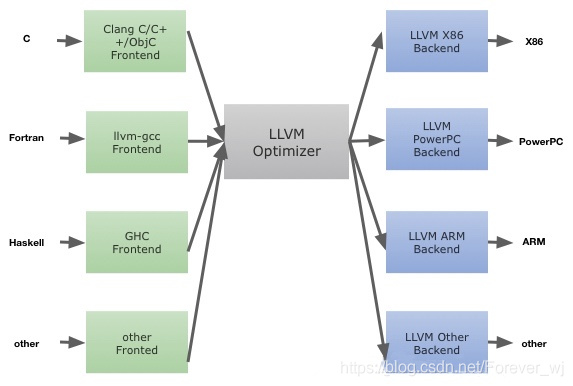
\includegraphics[scale=0.4]{llvmDesign.jpg}
% \end{center}
% \caption{Dizajn kompilatorske infrastrukture LLVM}
% \label{fig:exploded}
% \end{figure}


\textit{Clang} predstavlja prednji deo (\textit{eng.~frontend}) kompilatorske infrastrukture LLVM za familiju jezika u \v{c}ijoj se osnovi nalazi programski jezik C (C, C++, Objective C/C++, OpenCL ...). Pored optimizacija i efikasnog generisanja LLVM međukoda, \textit{Clang} odlikuje i ekspresivnost dijagnostike odnosno kvalitet poruka upozorenja i grešaka prijavljenih za izvorni k\^{o}d. \textit{Clang} se sastoji od vi\v{s}e biblioteka od kojih su najznačajnije nabrojane u nastavku.

\begin{description}
  \item[Biblioteka \texttt{clangLex}] sadr\v{z}i nekoliko usko povezanih klasa koje implementiraju pretprocesiranje i leksi\v{c}ku analizu izvornog koda. Najva\v{z}nije klase u okviru ove biblioteke
       su \texttt{Lexer} i  \texttt{Preprocessor}.
       \texttt{Preprocessor} pru\v{z}a mogućnost uslovne kompilacije, uključivanja datoteka zaglavlja i proširenja makroa.
       \texttt{Lexer} kreira niz tokena od izvornog koda.
  \item[Biblioteka \texttt{clangParse}]
        obrađuje niz tokena dobijenih leksi\v{c}kom analizom i od njih kreira \v{c}vorove apstraktnog sintaksi\v{c}kog stabla. Ova biblioteka koristi funkcionalnosti 
        biblioteke \texttt{clangSema} kako bi ispitala semanti\v{c}ku validnost sintaksnih konstrukta (niza tokena) od kojih kreira \v{c}vorove apstraktnog sintaksi\v{c}kog stabla.
        Parser kompilatora \textit{Clang} je implementiran kao parser rekurzivnog spuštanja (eng.~\textit{recursive-descent parser}), odnosno analizira izvorni k\^{o}d od vrha ka dnu nizom rekurzivnih funkcija \cite{LLVMCoreLibraries}.
  \item[Biblioteka \texttt{clangAST}]
        implementira algoritme i strukture podataka koje parser koristi za izgradnju apstraktnog sintaksi\v{c}kog stabla. Specifična je po strukturi čvorova koji podsećaju na izvorni C++ k\^{o}d što je čini pogodnom za kreiranje alata za refaktorisanje koda i statičku analizu. S obzirom da se ova biblioteka koristi u okviru alata \textit{AutoFix}, opisana je detaljnije u poglavlju \ref{sec:clangASTSec}.
  \item[Biblioteka \texttt{clangSema}]
        vrši semantičku analizu programa tokom parsiranja. Ova biblioteka proverava da li je k\^{o}d napisan u skladu sa sistemom tipova koji standard jezika propisuje. Za razliku od uobi\v{c}ajenog na\v{c}ina implementacije provere tipova, obilaskom apstraktnog sintaksi\v{c}kog stabla nakon parsiranja, biblioteka \texttt{clangSema} implementira proveru tipova zajedno sa generisanjem \v{c}vorova apastraktong sintaksi\v{c}kog stabla \cite{LLVMCoreLibraries}. Ova biblioteka usko je povezana sa bibliotekama \texttt{clangParse} i \texttt{clangAST}.
  \item[Biblioteka \texttt{clangCodeGen}]
        generiše LLVM međukod. Ova biblioteka obilazi apstraksno sintaksi\v{c}ko stablo i na osnovu njegovog sadr\v{z}aja generi\v{s}e instrukcije
        LLVM međukoda koje implementiraju pona\v{s}anje opisano u stablu \cite{LLVMCoreLibraries}.
\end{description}

% \begin{figure}[!ht]
%   \centering
%   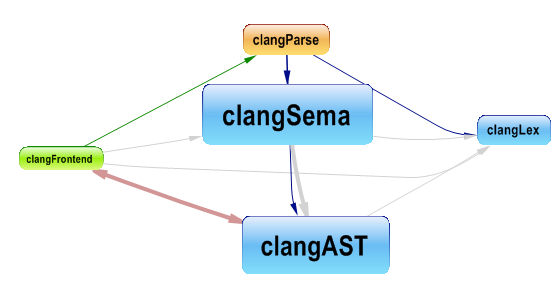
\includegraphics[width=1\textwidth]{ClangBiblioteke.png}
%   \caption{Odnos osnovnih biblioteka Clang-a.}
%   \label{fig:grafikon}
% \end{figure}

\section{Biblioteka \texttt{clangAST}}
\label{sec:clangASTSec}
U računarstvu, \textbf{apstraktno sintaksi\v{c}ko stablo}, ili samo \textbf{sintaksi\v{c}ko stablo}, je drvoidna reprezentacija apstraktne sintaksne strukture izvornog koda napisanog u programskom jeziku. Svaki čvor stabla predstavlja konstrukt koji se pojavljuje u izvornom kodu.
Sintaksa je apstraktna u smislu da ne sadr\v{z}i svaki detalj koji se pojavljuje u sintaksi, ali sadr\v{z}i sve detalje neophodne za nedvosmislen prikaz izvornog koda.

Ekspresivnost dijagnostike kompilatora \textit{Clang} i jednostavnost kreiranja mo\'{c}nih alata za stati\v{c}ku analizu u velikoj meri oslanja se na dizajn biblioteke \texttt{clangAST}. Struktura apstraktnog sintaksi\v{c}kog stabla mo\v{z}e se jednostavno ispisati na standardni izlaz opcijom komandne linije \texttt{-ast-dump}. Slika \ref{fig:ASTSlika} predstavlja tekstualnu reprezentaciju apstraktnog sintaksi\v{c}kog stabla generisanog za k\^{o}d iz fajla \texttt{hello.cpp} prikazanog na listingu \ref{lst:label4}.
\\

\begin{lstlisting}[style=customc, caption={K\^{o}d \v{c}ije je apstraktno sintaksi\v{c}ko stablo prikazano na slici \ref{fig:ASTSlika}.},label=lst:label4]
int main(){
  int a = 4;
  int b = 5;
  int result = a * b + 8;
}
\end{lstlisting}

% primer korišćenja slike
\begin{figure}[!ht]
  \centering
  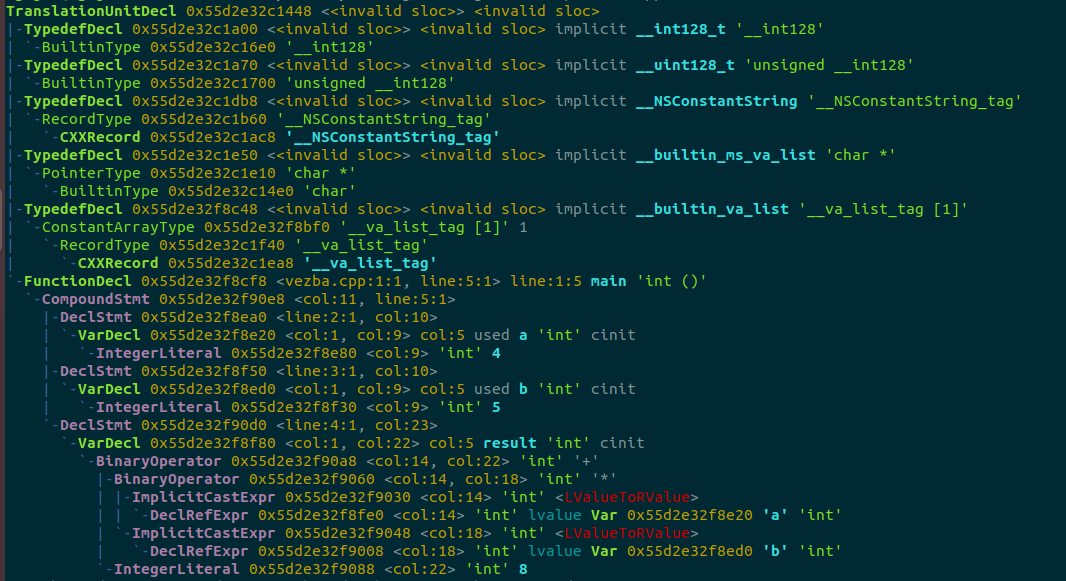
\includegraphics[width=1.0\textwidth]{ASTImage.png}
  \caption{Apstraktno sintaksi\v{c}ko stablo za k\^{o}d iz listinga \ref{lst:label4} koje je generisano komandom: \texttt{clang -Xclang -ast-dump hello.c}.}
  \label{fig:ASTSlika}
\end{figure}

\v{C}vorovi od kojih je izgrađeno apstraktno sintaksi\v{c}ko stablo predstavljaju apstrakciju sintaksnih struktura iz samog jezika.
Svi \v{c}vorovi apstraktnog sintaksi\v{c}kog stabla kompilatora \textit{Clang} nasleđuju jednu od tri osnovne (bazne) klase:
\begin{itemize}
  \item \texttt{Decl}
  \item \texttt{Stmt}
  \item \texttt{Type}
\end{itemize}
Ove klase redom opisuju deklaracije, naredbe i tipove iz familije jezika u \v{c}ijoj se osnovi nalazi jezik C.
Na primer, klasa \texttt{IfStmt} opisuje naredbe \texttt{if} u jeziku i direktno nasleđuje klasu \texttt{Stmt}. Sa druge strane, klase \texttt{FunctionDecl} i \texttt{VarDecl}, koje se koriste za opisivanje deklaracija i definicija funkcija i varijabli, ne nasleđuju dikertno klasu \texttt{Decl} ve\'{c} nasleđuju vi\v{s}e njenih podklasa.
\par
\v{C}vorovi apstraktnog sintaksi\v{c}kog stabla dugog \v{z}ivotnog veka (eng.~\textit{long-lived}), kao \v{s}to su tipovi i deklaracije, \v{c}uvaju se u klasi \texttt{ASTContext}. Ova klasa
omogu\'{c}ava upotrebu tih \v{c}vorova tokom semanti\v{c}ke analize programa. \texttt{ASTContext} takođe \v{c}uva referencu na objekat klase \texttt{SourceManager}. Ovo je
\v{c}ini pogodnom i za prikupljanje informacija o lokacijama iz izvornog fajla koje odgovaraju \v{c}vorovima iz apstraktnog sintaksi\v{c}kog stabla. Ovakve informacije posebno su korisne za kreiranje
preciznih poruka dijagnostike koda.

\subsection{Klasa \texttt{Type}}
  Klasa \texttt{Type} igra va\v{z}nu ulogu u ekspresivnosti dijagnostike kompilatora \textit{Clang}, a samim tim i u kvalitetu alata za stati\v{c}ku analizu. Ova klasa omgu\'{c}ava da poruke upozorenja sadr\v{z}e precizne informacije o tipovima. Na primer, upozorenja vezana za k\^{o}d koji koristi tip \texttt{std::string}, ispisa\'{c}e ba\v{s} taj tip u svojim porukama umesto tipa koji \texttt{std::string} predefini\v{s}e, a to je \texttt{std::basic\_string<char, ... >}. Iza ove funkcionalnosti stoji ideja kanonskih tipova.
  
  \par
  Svaka instanca klase \texttt{Type} sadr\v{z}i pokaziva\v{c} na svoj kanonski tip. Za jednostavne tipove koji nisu definisani kori\v{s}\'{c}enjem naredbe \texttt{typedef}, pokaziva\v{c} na kanonski tip \'{c}e zapravo pokazivati na sebe. Za tipove \v{c}ija struktura uklju\v{c}uje naredbu \texttt{typedef}, kanonski pokaziva\v{c} pokaziva\'{c}e na strukturno ekvivalentan tip bez naredbe \texttt{typedef}.
  Na primer, kanonski tip tipa \texttt{int *} sa listinga \ref{lst:label5}  bi\'{c}e sam taj tip, dok \'{c}e kanonski tip za \texttt{foo *} biti \texttt{int *}.

\begin{lstlisting}[style=customc, caption={Primer kanonskog tipa (\texttt{int *}) i tipa koji nije kanonski (\texttt{foo *}). },label=lst:label5]
  int *a;
  typedef int foo;
  foo *b;
\end{lstlisting}
  Ovakav dizajn omogu\'{c}ava semanti\v{c}kim proverama da donose zaklju\v{c}ke direktno o pravom tipu ignori\v{s}u\'{c}i naredbe \texttt{typedef}, kao i efikasno poređenje strukturne identi\v{c}nosti tipova.

  \par
  Klasa \texttt{Type} ne sadr\v{z}i informacije o kvalifikatorima tipova kao \v{s}to su \texttt{const}, \texttt{volatile}, \texttt{restrict} itd. Ove informacije enkapsulirane su u klasi \texttt{QualType} koja predstavlja par pokaziva\v{c}a na tip (objekat klase \texttt{Type}) i bitova koji predstavljaju
  kvalifikatore. \v{C}uvanje kvalifikatora u vidu bitova omogu\'{c}ava veoma efikasno dohvatanje, dodavanje i brisanje kvalifikatora za tip. Postojanje ove klase smanjuje upotrebu hip memorije time \v{s}to se ne moraju kreirati duplikati tipova sa razli\v{c}itim kvalifikatorima. Na hipu se alocira jedan tip, a zatim 
  svi kvalifikovani tipovi pokazuju na alocirani tip na hipu sa dodatim kvalifikatorima \cite{CFEWebsite}.

\subsection{AST-posetioci}
AST-posetioci (eng.~\textit{AST-visitors}) implementiraju mehanizam obilaska apstraktnog sintaksi\v{c}kog stabla kompilatora \textit{Clang}, odnosno pru\v{z}aju interfejs \footnote{U ovom radu pod terminom \textit{interfejs} smatra se skup metoda ili funkcija koje pru\v{z}aju pristup određenim funkcionalnostima i omogu\'{c}avaju njihovu upotrebu.}
za posetu svakog \v{c}vora u apstraktnom sintaksi\v{c}kom stablu.
Funkcionalnost AST-posetioca implementirana je u okviru šablonske klase  \texttt{RecursiveASTVisitor<Deri\-ved>}.
Objekat ove klase posećuje svaki čvor apstraktnog sintaksi\v{c}kog stabla obilaskom u dubinu.
AST-posetilac je svaka potklasa klase \texttt{RecursiveASTVisitor<Der\-ived>}.
Klasa \texttt{RecursiveASTVisitor<\-Derived>} omogu\'{c}ava obavljanje tri odvojena zadatka:

\begin{enumerate}
\item Obilazak apstraktnog sintaksi\v{c}kog stabla, odnosno pose\'{c}ivanje svakog \v{c}vora.
\item Obilazak klasne hijerarhije za \v{c}vor, počevši od dinamičkog tipa čvora do klase na vrhu hijerarhije (npr. \texttt{Stmt}, \texttt{Decl} ili \texttt{Type}).
\item Za datu kombinaciju \textit{(čvor, klasa)} omogu\'{c}ava pozivanje funkcije koje korisnik može predefinisati kako bi izvr\v{s}io analizu čvora.
\end{enumerate}
Ova tri zadatka obavljaju tri grupe metoda, redom:
\begin{enumerate}
  \item Metode \texttt{TraverseDecl(Decl *x)}, \texttt{TraverseStmt(Stmt *x)} i \texttt{TraverseType\-(QualType x)} implementiraju obilazak, redom, deklaracija, izraza i tipova u okviru apstraktnog sintaksi\v{c}kog stabla. Ovo su ulazne tačke za obilazak apstraktnog sintaksi\v{c}kog stabla sa korenom u čvoru \texttt{x}. Ove metode pozivaju metod \\ \texttt{TraverseFoo(Foo *x)}, gde je \texttt{Foo} dinamički tip od \texttt{*x}, koji poziva metod \\ \texttt{WalkUpFromFoo(x)}, a zatim rekurzivno posećuje decu čvora \texttt{x}. \\
  Na primer, ukoliko je dinami\v{c}ki tip od \texttt{*x} tip \texttt{CXXRecordDecl}, metod \\ \texttt{TraverseDecl(Decl *x)} \\ \'{c}e pozvati metod \\ \texttt{TraverseCXXRecordDecl(CXXRecordDecl *x)} \\ koji \'{c}e pozvati metod \\ \texttt{WalkUpFromCXXRecordDecl(CXXRecordDecl *x)}. 

\item Metod \texttt{WalkUpFromFoo(Foo *x)} obilazi klasnu hijerarhiju za \v{c}vor \texttt{x}. Ovaj metod ne pokušava odmah da poseti decu čvora \texttt{x}, umesto toga prvo zove \texttt{WalkUpFromBar(x)}, gde je \texttt{Bar} direktna nadklasa klase \texttt{Foo}, i tek onda zove \texttt{VisitFoo(x)}. \\
Na primer, \texttt{WalkUpFromCXXRecordDecl(CXXRecordDecl *x)} poziva \\ \texttt{WalkUpFromRecordDecl(x)} i \texttt{VisitCXXRecordDecl(x)}.
\item Metod \texttt{VisitFoo(Foo *x)} analizira \v{c}vor \texttt{x} tipa \texttt{Foo}. \\Na primer, metod \texttt{VisitCXXRecordDecl(CXXRecordDecl *x)} mo\v{z}e biti predefinisan kako bi se analizirao \v{c}vor \texttt{x} tipa \texttt{CXXRecordDecl}.
\end{enumerate}
Za ove tri grupe metoda defini\v{s}e se naredni poredak: \texttt{Traverse > WalkUpFrom > Visit}. Ovaj poredak ozna\v{c}ava da metod mo\v{z}e pozvati samo metode iz svoje grupe metoda ili iz grupe metoda direktno ispod nje. Metod ne mo\v{z}e pozvati metode iz grupe iznad \cite{visitors}. Na primer, metod \texttt{WalkUpFrom} mo\v{z}e pozvati metode iz svoje grupe i grupe \texttt{Visit} ali 
ne mo\v{z}e pozvati metode iz grupe \texttt{Traverse}. Metode iz grupe \texttt{Traverse} ne mogu pozvati metode iz grupe \texttt{Visit}, jer iako je grupa metoda \texttt{Visit} u definisanom poretku ispod grupe metoda \texttt{Traverse}, između te dve grupe metoda nalazi se grupa \texttt{WalkUpFrom}.
Drugim re\v{c}ima, u definisanom poretku grupa metoda \texttt{Visit} nije direktno ispod grupe metoda \texttt{Traverse}.

\subsection{Primer implementacije AST-posetioca}
Da bi se izvršila analiza izvornog koda pomoću AST-posetioca potrebno je naslediti klasu 
 \texttt{RecursiveASTVisitor<Derived>} i predefinisati željene metode \texttt{Visit} u okviru nje. Ukoliko je metodama \texttt{Visit} pronađen nepravilan konstrukt izvornog koda mo\v{z}e se prijaviti upozorenje. Na listingu \ref{lst:visitor} prikazan je primer posetioca. Metod \texttt{VisitEnumDecl} (linija 6) \'c{e} biti pozvan nad svim objektima klase \texttt{EnumDecl} u apstraktnom sintaksi\v{c}kom stablu. U okviru nje, proverava se da li deklaracija koristi \texttt{enum class} sintaksu, odnosno da li su konstante u okviru nabrajanja definisane u svom unutra\v{s}njem opsegu. Ukoliko sintaksa \texttt{enum class} nije kori\v{s}\'{c}ena pri deklaraciji, lokacija ove deklaracije, ukoliko je validna, ispisuje se na standardni izlaz (linija 13).

\begin{lstlisting}[style=customc,  caption={Primer posetioca koji pose\'{c}uje sve deklaracije nabrajanja i ispisuje lokaciju onih koji nisu deklarisani sintaksom \texttt{enum class}.},label=lst:visitor]
class FindUnscopedEnumVisitor
    : public RecursiveASTVisitor<FindUnscopedEnumVisitor> {
public:
  explicit FindUnscopedEnumVisitor(ASTContext *Context) : Context(Context) {}

  bool VisitEnumDecl(EnumDecl *ED) {
    if (!ED->isScopedUsingClassTag()) {
      // Get declaration location.
      FullSourceLoc FullLocation =
          Context->getFullLoc(ED->getBeginLoc());
      // Check if location is valid.
      if (FullLocation.isValid())
        llvm::outs() << "Found declaration at "
                     << FullLocation.getSpellingLineNumber() << ":"
                     << FullLocation.getSpellingColumnNumber() << "\n";
    }
    return true;
  }

private:
  ASTContext *Context;
};
\end{lstlisting}

\section{Dijagnostika u okviru kompilatora \textit{Clang}}
\label{sec:diagnostics}

Sistem dijagnostike u kompilatoru \textit{Clang} igra va\v{z}nu ulogu u tome kako kompilator komunicira sa korisnikom. Pod dijagnostikom
smatraju se upozorenja i gre\v{s}ke koje kompilator prijavljuje za k\^{o}d koji je neispravan ili \v{c}ija je ispravnost sumnjiva. \par
U kompilatoru \textit{Clang} svaka dijagnostika sadr\v{z}i jedinstveni identifikator, poruku na Engleskom jeziku koja opisuje problem u kodu, lokaciju u izvornom kodu (objekat klase \texttt{SourceLocation}) na koju se dijagnostika odnosi i nivo ozbiljnosti (eng.~\textit{severity}) dijagnostike (na primer, upozorenje ili gre\v{s}ka). \par Objekat klase \texttt{SourceLocation} omogu\'{c}ava ispisivanje putanje do izvornog fajla u kome se nalazi k\^{o}d, linije koda i kolone u okviru linije. Ove informacije ispisuju se u obliku \texttt{putanja\_do\_fajla:broj\_linije:broj\_kolone}. Na lokaciju u izvornom fajlu na koju se dijagnostika odnosi, u okviru ispisane poruke, pokaziva\'{c}e karakter \hspace*{1mm} \texttt{\^}. Opciono, pored lokacije na koju se odnosi, dijagnostika mo\v{z}e sadr\v{z}ati i opseg lokacija na koji se odnosi (objekat klase \texttt{SourceRange}). Opseg \'{c}e u poruci biti podvu\v{c}en karakterima \hspace{2mm} \texttt{\~} \cite{CFEWebsite}.
\par
Na slici \ref{fig:warning} prikazan je primer ispisa upozorenja na standardni izlaz. Upozorenje sadr\v{z}i informacije o lokaciji, nivo upozorenja, opseg i poruku upozorenja.

\begin{figure}[!h]
\begin{center}
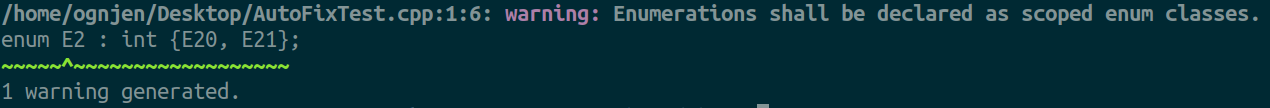
\includegraphics[scale=0.225]{warning.png}
\end{center}
\caption{Primer ispisa upozorenja na standardni izlaz.}
\label{fig:warning}
\end{figure}

\subsection{Predlozi za ispravljanje koda}

Kompilator \textit{Clang} podr\v{z}ava mehanizam kojim se za neispravan k\^{o}d, na koji se odnosi dijagnostika, mogu ispisati predlozi za ispravljanje tog koda (eng.~\textit{fixit hint}). Ovaj mehanizam podr\v{z}an je kroz klasu \texttt{FixItHint}.
\par
Instance klase \texttt{FixItHint} dodaju se ve\'{c} kreiranoj dijagnostici. Objekti ove
klase mogu biti kreirani jednim od slede\'{c}a tri konstruktora:

\begin{itemize}
\item \texttt{FixItHint::CreateInsertion(Loc, Code)} --- Kreira objekat koji predla\v{z}e da se k\^{o}d (predstavljen stringom) \texttt{Code} umetne ispred lokacije \texttt{Loc}.
\item \texttt{FixItHint::CreateRemoval(Range)} --- Kreira objekat koji predla\v{z}e da se izbri\v{s}e k\^{o}d iz opsega \texttt{Range}.
\item \texttt{FixItHint::CreateReplacement(Range, Code)} --- Kreira objekat koji predla\v{z}e da se izbri\v{s}e k\^{o}d iz opsega \texttt{Range} i da se zameni sa kodom \texttt{Code}.
\end{itemize}

Na slici \ref{fig:fixit} prikazan je ispis upozorenja sa predlogom za ispravljanje koda na standardni izlaz. Na slici je prikazana lokacija
ispred koje treba umetnuti klju\v{c}nu re\v{c} \texttt{class} kako bi k\^{o}d bio ispravan.

\begin{figure}[!h]
\begin{center}
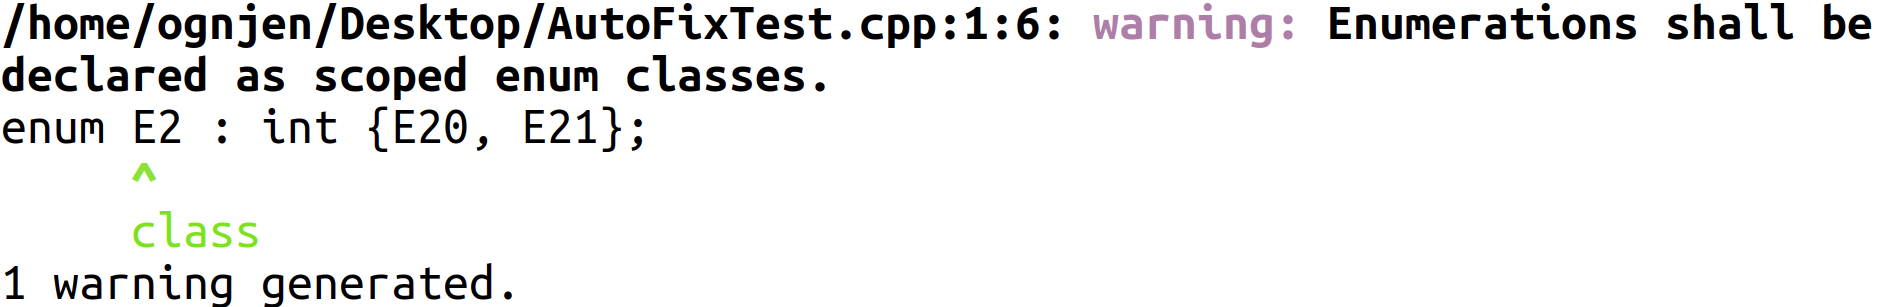
\includegraphics[scale=0.225]{fixit.png}
\end{center}
\caption{Primer ispisa upozorenja sa predlogom za ispravljanje koda na standardni izlaz.}
\label{fig:fixit}
\end{figure}

\subsection{Klasa \texttt{DiagnosticConsumer}}

Klasa \texttt{DiagnosticConsumer} u okviru kompilatora \textit{Clang} ima ulogu da obradi (konzumira) dijagnostiku prijavljenu
za izvorni k\^{o}d. Ovo je apstraktna klasa i svaka klasa koje je nasleđuje treba da implementira konkretan vid obrade dijagnostike. \par
Na primer, jedan vid obrade dijagnostike jeste formatiranje poruka dijagnostike i ispisivanje poruka zajedno sa informacijama o lokaciji i opsegu.
Ovakvu obradu vr\v{s}i klasa \texttt{TextDiagnosticPrinter}, potklasa klase \texttt{DiagnosticConsumer}.
Ispisivanje dijagnostike nije jedini vid obrade dijagnostike, niti je neophodan. Na primer, dijagnostika se mo\v{z}e obraditi
tako \v{s}to \'{c}e za svaku kreiranu dijagnostiku biti provereno da li je o\v{c}ekivana i ukoliko nije, sprove\v{s}\'{c}e se određene akcije.
Ovakav vid obrade dijagnostike vr\v{s}i klasa \texttt{VerifyDiagnosticConsumer}, potklasa klase \texttt{DiagnosticConsumer} \cite{CFEWebsite}.

Klasa \texttt{DiagnosticConsumer} defini\v{s}e nekoliko metoda u svrhu obrade dijagnostike. U ovom radu kori\v{s}\'{c}ene su metode:
\begin{itemize}
\item \texttt{HandleDiagnostic} --- poziva se nakon kreiranja svake dijagnostike u okviru kompilatora i slu\v{z}i za obradu te dijagnostike. 
\item \texttt{finish} --- poziva se nakon \v{s}to su kreirane i obrađene sve dijagnostike u okviru kompilatora i slu\v{z}i za dodatnu obradu celokupne dijagnostike.
\end{itemize}

\subsection{Klasa \texttt{DiagnosticsEngine}}

U okviru kompilatora \textit{Clang} dijagnostika se prijavljuje upotrebom klase \texttt{Diagno\-sticsEngine}. Ova klasa slu\v{z}i 
za kreiranje dijagnostike i prosleđivanje dijagnostike objektu klase \texttt{DiagnosticConsumer}. Dijagnostika se kreira pozivanjem metode \texttt{Report}. Ovaj metod kao argumente dobija informacije potrebne za kreiranje dijagnostike, kao \v{s}to su lokacija i poruka i koristi ih da kreira objekat klase \texttt{DiagnosticBuilder}. Kreirani objekat predstavlja povratnu vrednost metode \texttt{Report}. \par
\texttt{DiagnosticBuilder} predstavlja malu, pomo\'{c}nu klasu za prijavljivanje dijagnostike. Ova klasa olak\v{s}ava prosleđivanje
dodatnih informacija prilikom kreiranja dijagnostike, kao \v{s}to su opsezi ili predlozi izmene koda. Prosleđivanje dodatnih informacija se vr\v{s}i upotrebom operatora \texttt{<<} koji klasa \texttt{DiagnosticBuilder} defini\v{s}e. Operator \texttt{<<} kao argument prima dodatne informacije, kao \v{s}to su objekti klase \texttt{SourceRange} ili \texttt{FixItHint}. Dijagnostika kreirana metodom
\texttt{Report} se prosleđuje objektu klase \texttt{DiagnosticConsumer} prlikom uni\v{s}tavanja, odnosno u destruktoru kreiranog objekta klase \texttt{DiagnosticBuilder}. 


\subsection{Primer prijavljivanja dijagnostike u kompilatoru \textit{Clang}}

Na listingu \ref{lst:dijagnostika} prikazana je funkcija \texttt{emitWarningWithHintInsertion} kojom se prijavljuje
upozorenje zajedno sa predlogom za ispravljanje koda. Upozorenje se prijavljuje pozivom metode \texttt{Report} (linija 10). Ovaj metod kao argumente
dobija lokaciju za koju treba prijaviti dijagnostiku (\texttt{diagLoc}) i jedinstveni identifikator (\texttt{ID}). Identifikator je kreiran, pozivom metode \texttt{getCustomDiagID(DiagnosticIDs\-::Warning, msg)}, za dijagnostiku sa nivoom ozbiljnosti upozorenja i porukom \texttt{msg} (linija 7). Metod \texttt{Report} na osnovu ovih informacija kreira i vra\'{c}a
objekat klase \texttt{DiagnosticBui\-lder} kom se prosleđuje kreirani objekat klase \texttt{FixItHint} (linija 10). Upozorenje \'{c}e biti prosleđeno
objektu klase \texttt{DiagnosticConsumer} odmah nakon dodavanja predloga za ispravljanje koda s obzirom da objekat klase \texttt{DiagnosticBuilder}
nije vezan ni za jednu promenljivu i odmah \'{c}e biti uni\v{s}ten.

\begin{lstlisting}[style=customc, caption={Primer prijavljivanja dijagnostike u kompilatoru \textit{Clang}.}, label=lst:dijagnostika]
void emitWarningWithHintInsertion(DiagnosticsEngine &DE, 
                                  std::string &msg,
                                  std::string &str, 
                                  SourceLocation insertLoc,
                                  SourceLocation diagLoc) {
  unsigned ID =
      DE.getDiagnosticIDs()->getCustomDiagID(DiagnosticIDs::Warning
                                             ,msg);
  FixItHint hint = FixItHint::CreateInsertion(insertLoc, str);
  DE.Report(diagLoc, ID) << hint;
}
\end{lstlisting}

\section{AST-upariva\v{c}i}
\label{sec:matchers}

AST-upariva\v{c} (ili samo upariva\v{c}) je objekat \v{s}ablonske klase \texttt{Matcher}. Upariva\v{c}i slu\v{z}e za jednostavno
pronala\v{z}enje \v{c}vorova apstraktnog sintaksi\v{c}kog stabla koji imaju određene \v{z}eljene karakteristike. Pronađeni \v{c}vorovi se 
\v{c}uvaju u odgovaraju\'{c}im strukturama podataka kako bi se kasnije mogli analizirati. \v{Z}eljene karakteristike \v{c}vorova koje upariva\v{c} treba da pronađe se zadaju prilikom kreiranja upariva\v{c}a kori\v{s}\'{c}enjem izraza za uparivanje (eng.~\textit{match expressions}).
Ovo su izrazi jezika specijalne namene implementiranog u okviru biblioteke AST-upariva\v{c}a (eng.~\textit{LibASTMatchers}). Ovaj jezik pru\v{z}a mogu\'{c}nost kreiranja predikata nad apstraktnim sintaksnim stablom.

\par
Na primer, za kreiranje upariva\v{c}a koji izdvaja sve deklaracije enumeratora iz apstraktnog sintaksi\v{c}kog stabla mo\v{z}e se koristiti izraz za uparivanje \texttt{enumDecl()}. Ukoliko prilikom uparivanja treba ignorisati deklaracije iz zaglavlja, izraz za uparivanje mo\v{z}e se pro\v{s}iriti izrazom \texttt{isExpansionIn\-MainFile()}. Izraz \\ \texttt{enumDecl(isExpansionInMainFile())} \\ kreira\'{c}e upariva\v{c} koji slu\v{z}i za izdvajanje deklaracija enumeratora iz glavnog (\texttt{.cpp}) fajla \cite{ASTMatcherReference, MatchingClangAST}.

Nakon uparivanja, nad izdvojenim konstruktom mo\v{z}e se vr\v{s}iti dodatna analiza, na primer ispitivanje saglasnosti konstrukta sa pravilom standarda za pravilno pisanje C++ koda.
S obzirom da upariva\v{c}i \v{c}esto predstavljaju kompoziciju vi\v{s}e upariva\v{c}a, zgodno je imati mogu\'{c}nost adresiranja svakog podrezultata (rezultata svakog od upariva\v{c}a u kompoziciji) zasebno. Na primer, upariva\v{c} mo\v{z}e izdvajati deklaracije enumeratora, ali samo one koje defini\v{s}u i neku konstantu u okviru nabrajanja, odnosno deklaracije koje imaju potomka u stablu tipa \texttt{EnumConstantDecl}. U ovom slu\v{c}aju
zgodno je da se u okviru analize izdvojenog \v{c}vora, odnosno deklaracije enumeratora, mo\v{z}e direktno analizirati njegov potomak, konstanta u okviru nabrajanja, bez potrebe da se ovaj potomak ponovo tra\v{z}i u apstraktnom sintaksi\v{c}kom stablu.

U svrhu adresiranja rezultata pretrage, upariva\v{c}i se mogu "vezati" (eng.~\textit{binding}) za određeni string. Na primer, izraz \\
\texttt{enumDecl(hasDescendant(enumConstantDecl().bind("EnumConstNode")))} \\
\hspace*{9cm}\texttt{.bind("EnumNode")} \\ će vezati izdvojene deklaracije enumeratora za string \texttt{"EnumNode"}, dok \'{c}e konstante vezati za string \texttt{EnumConstNode}. Rezultati uparivanja predstavljeni su kao objekti klase \texttt{MatchResult}. Iz promenljive \texttt{Result} koja predstavlja objekat klase \texttt{MatchResult}, \v{c}vor koji predstavlja deklaraciju enumeratora
mo\v{z}e se dobiti izrazom \\ \texttt{auto ED = Result.Nodes.getNodeAs<EnumDecl>("EnumNode")} \\
dok se \v{c}vor koji predstavlja deklaraciju konstante u okviru nabrajanja mo\v{z}e dobiti izrazom \\ \texttt{auto ECD = Result.Nodes.getNodeAs<EnumConstantDecl>("EnumConstNode")}.\\ Dobijeni \v{c}vorovi se onda mogu koristiti u svrhu analiziranja
koda koji predstavljaju.

\par
Nakon formulisanja izraza za uparivanje kreirani upariva\v{c} se pokre\'{c}e nad apstraktnim sintaksnim stablom. Ovo se posti\v{z}e pozivanjem metode \texttt{matchAST()} klase \texttt{MatchFinder}. 
Za obilazak koji \'{c}e izvr\v{s}iti objekat klase \texttt{MatchFinder} upariva\v{c}i se registruju zajedno sa objektima koji implementiraju povratni poziv upariva\v{c}a (eng.~\textit{match callback}). 
Ovo su objekti klase \texttt{MatchCallback} \v{c}iji metod \texttt{run(const MatchResult \&)} se poziva nakon svakog uspe\v{s}nog uparivanja 
upariva\v{c}a sa kojim je ovaj povratni poziv registrovan. Za implementaciju specifi\v{c}nog povratnog poziva treba implementirati klasu koja nasleđuje klasu \texttt{MatchCallback} i predefinisati metod \texttt{run}. U okviru metode \texttt{run} mo\v{z}e se vr\v{s}iti dodatna analiza izdvojenih \v{c}vorova i po potrebi
prijavljivati dijagnostika vezana za k\^{o}d koji taj rezultat predstavlja. 
\subsection{Primer implementacije AST-upariva\v{c}a}
Na listingu \ref{lst:MatcherList} prikazan je primer upariva\v{c}a koji pronalazi sve deklaracije enumeratora koje ne koriste sintaksu \texttt{enum class}. Za ove enumeratore prijavljuje se upozorenje zajedno sa predlogom za ispravljanje koda u okviru funkcije \texttt{emitWarningWithHintInsertion} (linija 22). U funkciji \texttt{matchASTExample} kreiraju se upariva\v{c} (linija 33) i objekat klase povratnog poziva (linija 35). Nakon toga, upariva\v{c} se registruje za obilazak (linija 37) i pokre\'{c}e nad apstraktnim sintaksnim stablom pomo\'{c}u objekta klase \texttt{MatchFinder} (linija 39).

\begin{lstlisting}[style=customc,  caption={Primer upariva\v{c}a koji pronalazi sve deklaracije enumeratora koje ne koriste sintaksu \texttt{enum class}. Ovaj primer demonstrira i upotrebu klasa \texttt{MatchFinder}, \texttt{MatchCallback} i \texttt{MatchResult}. Funkcija \texttt{emitWarningWithHintInsertion} implementirana je na listingu \ref{lst:dijagnostika} i dostupna je kroz zaglavlje \texttt{EmitWarning.h}}, label=lst:MatcherList]
#include "EmitWarning.h"

// Callback class.
class A7_2_3 : public MatchFinder::MatchCallback {
public:
  A7_2_3(ASTContext &ASTCtx) : ASTCtx(ASTCtx) {}
  virtual void run(const MatchFinder::MatchResult &Result);

private:
  ASTContext &ASTCtx;
};

void A7_2_3::run(const MatchFinder::MatchResult &Result) {
  if (auto ED = Result.Nodes.getNodeAs<clang::EnumDecl>("A7_2_3_Matcher")) {
    // Check if declaration contains 'class' tag.
    if (!ED->isScopedUsingClassTag()) {
      // Create warning string.
      std::string msg =
          "Enumerations shall be declared as scoped enum classes.";
      std::string insStr = "class ";
      // Function for emitting warnings with fixit hints using diagnostics engine.
      emitWarningWithHintInsertion(
          ASTCtx.getDiagnostics(), msg, insStr,
          ED->getSourceRange().getBegin().getLocWithOffset(5),
          ED->getLocation());
    }
  }
}

void matchASTExample(ASTContext *Context){
  MatchFinder Finder;
  // Create matcher.
  Matcher<Decl> Matcher = enumDecl(isExpansionInMainFile()).bind("A7_2_3_Matcher");
  // Create callback class.
  MatchCallback *Callback = new A7_2_3(Context);
  // Register matcher.
  Finder.addMatcher(Matcher, Callback);
  // Run matcher over AST.
  Finder.matchAST(Context);
}
\end{lstlisting}


\section{Interfejsi za akcije nad prednjim delom kompilatora}
\label{sec:interfejsi}

Akcije nad prednjim delom kompilatora omogu\'{c}avaju analizu i upotrebu rezultata i informacija koje pru\v{z}a prednji deo kompilatora. Ove informacije mogu biti korisne za kreiranje alata za refaktorisanje koda, stati\v{c}ku analizu, prikupljanje statistike i grafi\v{c}ko prezentovanje rezultata kompilatora. Takođe, igraju i klju\v{c}nu ulogu u samoj kompilaciji koda i deo su glavne proto\v{c}ne obrade (eng.~\textit{pipeline}) u kompilatorskoj infrastrukturi LLVM.
Ova funkcionalnost je efikasno i sistemati\v{c}no implementirana u okviru klasa \texttt{ASTConsumer}, \texttt{ASTFrontendAction} i njihovih potklasa.

\subsection{Klasa ASTConsumer}

\texttt{ASTConsumer} je apstraktna klasa koja omogu\'{c}ava izvr\v{s}avanje razli\v{c}itih akcija nad apstraktnim sintaksnim stablom nezavisno od toga kako je apstraktno sintaksi\v{c}ko stablo kreirano.
Akcije se mogu izvr\v{s}avati u razli\v{c}itim fazama tokom kreiranja apstraktnog sintaksi\v{c}kog stabla \cite{ASTToolTutorial}. Na primer, metod \\ \texttt{virtual void  HandleInlineFunctionDefinition (FunctionDecl *D)} \\ bi\'{c}e pozvan svaki put kada se zavr\v{s}i kreiranje umetnutih (eng.~\textit{inline}) funkcija prilikom kreiranja apstraktnog sintaksi\v{c}kog stabla. \texttt{ASTConsumer} defini\v{s}e niz sli\v{c}nih virtuelnih metoda koje predefini\v{s}u klase koje je nasleđuju. \par
Na slici \ref{fig:inhDiagram} prikazane su klase u okviru kompilatora \textit{Clang} koje nasleđuju klasu \texttt{ASTConsumer}. Klasa \texttt{CodeGenerator}, prikazana na slici,
generi\v{s}e LLVM međukod od apstraktnog sintaksi\v{c}kog stabla i predstavlja jedan od osnovnih delova u kompilatorskoj infrastrukturi LLVM, \v{s}to demonstrira zna\v{c}aj klase \texttt{ASTConsumer}. 

% \usepackage{float}
\begin{figure}[!h]
\begin{center}
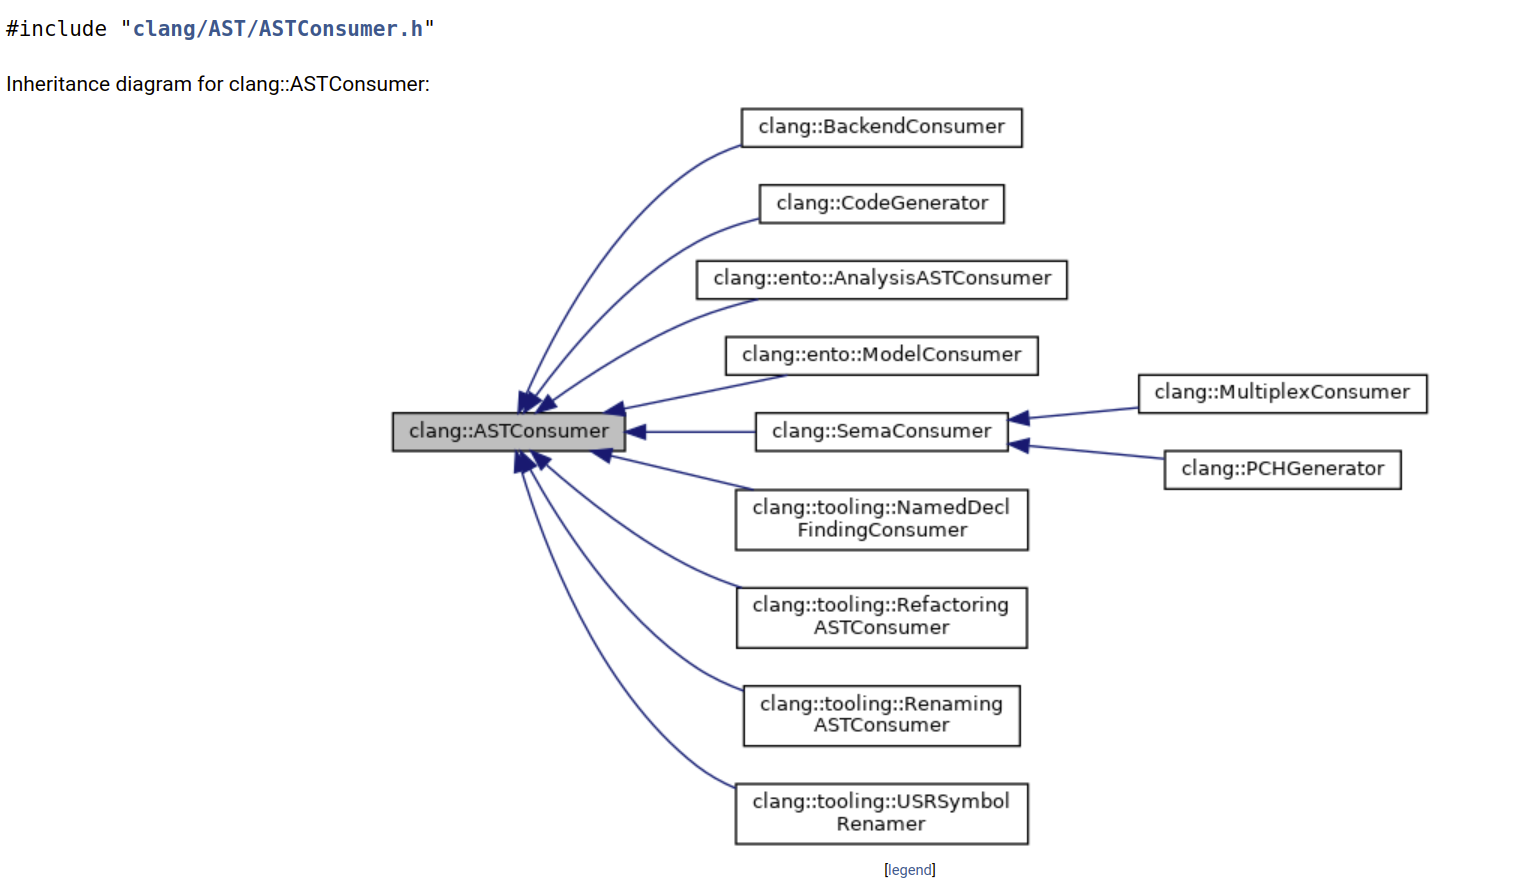
\includegraphics[scale=0.3]{ASTConsumer2.png}
\end{center}
\caption{Klase koje nasleđuju klasu \texttt{ASTConsumer} \cite{ASTConsumer}.}
\label{fig:inhDiagram}
\end{figure}

Klasa \texttt{ASTConsumer} korisna je i za kreiranje samostalnih alata za stati\v{c}ku analizu koji se zasnivaju na analizi apstraktnog sintaksi\v{c}kog stabla. U svrhu kreiranja alata mo\v{z}e se koristiti kombinacija upotrebe klase \texttt{ASTConsumer} sa mehanizmima za obilazak i obradu apstraktnog sintaksi\v{c}kog stabla kao \v{s}to su AST-posetioci i AST-upariva\v{c}i. \par
Za implementaciju specifi\v{c}ne akcije nad apstraktnim sintaksnim stablom
potrebno je implementirati potkasu klase \texttt{ASTConsumer} i u okviru nje predefinisati metod \\ \texttt{virtual void  HandleTranslationUnit(ASTContext \&Ctx)}.\\
Ovaj metod bi\'{c}e pozvan nakon \v{s}to je kreirano apstraktno sintaksi\v{c}ko stablo za jedinicu prevođenja, odnosno u trenutku kada je celokupno apstraktno sintaksi\v{c}ko stablo za jedinicu prevođenja dostupno.
U okviru njega, nad asptraktnim sintaksnim stablom, mo\v{z}e se pozvati AST-upariva\v{c} koji \'{c}e izvr\v{s}iti obilazak i analizu apstraktnog sintaksi\v{c}kog stabla \cite{ASTConsumer}.

\subsection{Primer upotrebe klase \texttt{ASTConsumer}}
Na listingu \ref{lst:labelConsumer} prikazana je implementacija klase \texttt{AutoFixConsumer}. U okviru metode \texttt{HandleTranslationUnit}
poziva se funkcija za kreiranje i pokretanje upariva\v{c}a \texttt{matchASTExample} (linija 9). 

\begin{lstlisting}[style=customc,  caption={Implementacija klase \texttt{AutoFixConsumer}. Funkcija \texttt{matchASTExample} prikazana je na listingu \ref{lst:MatcherList} i dostupna je kroz zaglavlje \texttt{AutoFixMatchers.h}.}, label=lst:labelConsumer]
#include "clang/AST/ASTConsumer.h"
#include "AutoFixMatchers.h"

class AutoFixConsumer : public clang::ASTConsumer {
public:
  explicit AutoFixConsumer(ASTContext *Context) : Context(Context) {}

  virtual void HandleTranslationUnit(clang::ASTContext &Context) {
    matchASTExample(Context);
  }

  ASTContext *Context;
};
\end{lstlisting}

\subsection{Klasa ASTFrontendAction}

\texttt{FrontendAction} je apstraktna klasa za akcije koje izvr\v{s}ava prednji deo kompilatora (eng.~\textit{frontend}).
Klasa \texttt{FrontendAction} ima raznolike upotrebe, odnosno specijalizacije. Primer specijalizacija ove klase su \texttt{DumpCompiler\-OptionsAction}
koja omogu\'{c}ava ispisivanje opcija koje se mogu zadati kompilatoru i \texttt{PreprocessorFrontendAction} koja omogu\'{c}ava izvr\v{s}avanje akcija vezanih za pretprocesiranje izvornog koda. Međutim, naj\v{c}es\'{c}a upotreba ove klase vezana je za akcije koje se izvr\v{s}avaju nad apstraktnim sintaksnim stablom. U ovu svrhu koristi se apstraktna klasa \texttt{ASTFrontendAction} koja je direktna potklasa klase \texttt{FrontendAction}. \par
\texttt{ASTFrontendAction} predefini\v{s}e metod \texttt{executeAction} klase \texttt{FrontendAction}. U okviru ove metode pozivaju se funkcije za semanti\v{c}ku analizu i kreiranje apstraktnog sintaksi\v{c}kog stabla. Nad ovim apstraktnim sintaksnim stablom izvr\v{s}i\'{c}e se akcije implementirane u objektu klase \texttt{ASTConsumer} pridru\v{z}enom ovoj klasi.
Na slici \ref{fig:ASTAction} prikazane su klase u okviru kompilatora \textit{Clang} koje nasleđuju klasu \texttt{ASTFrontendAction}. Slika demonstrira raznolikost upotrebe ove klase. \par
Da bi se implementirala specifi\v{c}na akcija nad apstraktnim sintaksnim stablom, potrebno je implementirati klasu koja nasleđuje klasu \texttt{ASTFronendAction} i dodeliti joj objekat klase \texttt{ASTConsumer} koji implementira \v{z}eljenu akciju. Objekat se kreira i dodeljuje predefinisanjem metode \\ 
\texttt{unique\_ptr<ASTConsumer> CreateASTConsumer(CompilerInstance Compiler,} \\
\hspace*{9cm} \texttt{StringRef InFile)} \\ 
Ova metoda kao argumente dobiija instancu kompilatora \textit{Clang} i ime fajla za koji se kreira apstraktno sintaksi\v{c}ko stablo. Povratna vrednost metode je pokaziva\v{c} na kreirani objekat klase \texttt{ASTConsumer}.
\subsection{Primer upotrebe klase \texttt{ASTFrontendAction}}
Na listingu \ref{lst:ASTAction} prikazana je implementacija klase \texttt{AutoFixAction} koja izvr\v{s}ava akcije nad apstraktnim sintaksnim stablom.
Klasa \texttt{AutoFixAction} u okviru metode \texttt{CreateASTConsumer} (linija 6) kreira pokaziva\v{c} na objekat klase \texttt{AutoFixConsumer}.

\begin{lstlisting}[style=customc,  caption={Implementacija klase \texttt{AutoFixAction}. Klasa \texttt{AutoFixConstumer} prikazana je na listingu \ref{lst:labelConsumer} i dostupna je kroz zaglavlje \texttt{AutoFixConsumer.h}.}, label=lst:ASTAction]
#include "AutoFixConsumer.h"

class AutoFixAction : public clang::ASTFrontendAction {
public:
  virtual std::unique_ptr<clang::ASTConsumer>
  CreateASTConsumer(clang::CompilerInstance &Compiler, 
                    llvm::StringRef InFile) {
    return std::make_unique<AutoFixConsumer>(
                &Compiler.getASTContext(),
                Compiler.getSourceManager());
  }
};
\end{lstlisting}


\begin{figure}[h!]
\begin{center}
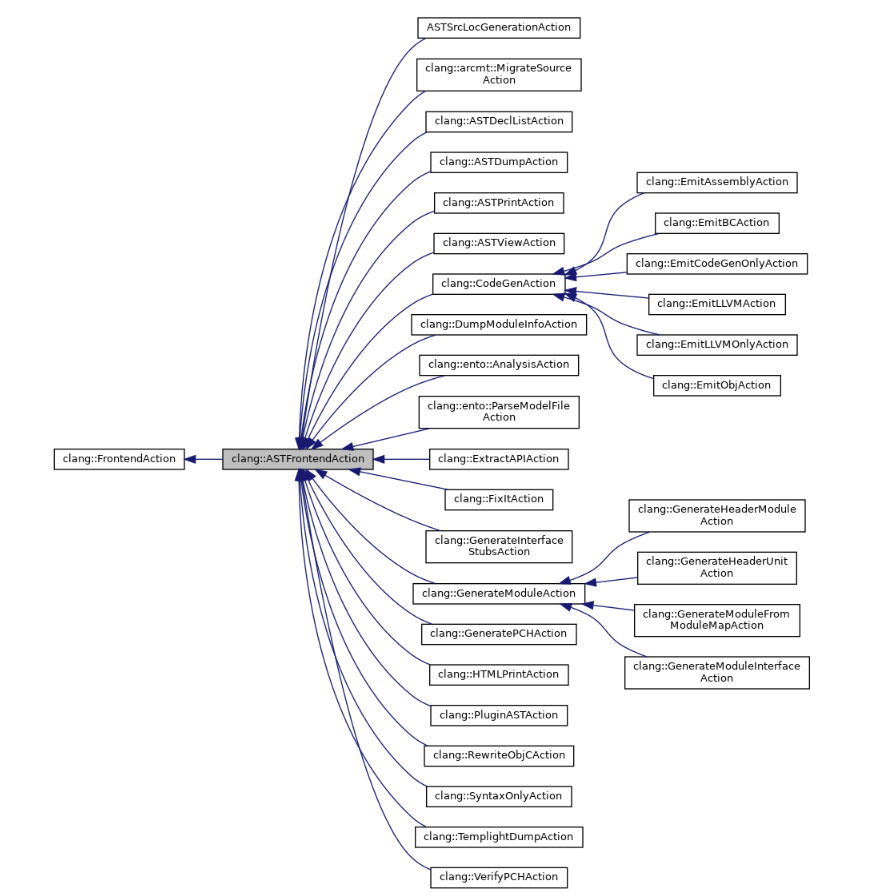
\includegraphics[scale=0.4]{ASTFrontendAction.png}
\end{center}
\caption{Klase koje nasleđuju klasu \texttt{ASTFrontendAction} \cite{ASTFrontendAction}.}
\label{fig:ASTAction}
\end{figure}



\section{Interfejsi za kreiranje alata}

Kompilatorska infrastruktura LLVM pru\v{z}a podr\v{s}ku za jednostavno kreiranje kvalitetnih alata za stati\v{c}ku analizu izvornog koda. Ovi alati
zasnivaju se na upotrebi interfejsa ka apstraktnom sintaksi\v{c}kom stablu kompilatora \textit{Clang} ili kori\v{s}\'{c}enjem stati\v{c}kog analizatora kompilatora \textit{Clang} (eng.~\textit{Clang Static Analyzer}) za potrebe simboli\v{c}kog izvr\v{s}avanja programa. \par Alati za stati\v{c}ku analizu mogu koristiti kombinaciju tehnika obrade apstraktnog sintaksi\v{c}kog stabla i simboli\v{c}kog izvr\v{s}avanja programa u zavisnosti od kompleksnosti analize koja je potrebna. Implementacija stati\v{c}ke analize obradom apstraktnog sintaksi\v{c}kog stabla je jeftinija po pitanju ra\v{c}unarskih resursa ali je ograni\v{c}ena informacijama dostupnim tokom kompilacije programa. \par 

 Kompilator \textit{Clang} pru\v{z}a vi\v{s}e infrastruktura za pisanje razli\v{c}itih vrsta softverskih alata koji koriste sintaksne i semanti\v{c}ke informacije o programu. U nastavku \'{c}e biti opisano nekoliko interfejsa koji se mogu koristiti u ovu svrhu zajedno sa njihovim prednostima i manama.


\begin{description}
\item[\texttt{LibClang}] je stabilni C interfejs visokog nivoa (eng.~\textit{high level}) ka kompilatoru \textit{Clang}. Ovaj interfejs pru\v{z}a parsiranje izvornog koda
i izagradnju apstraktnog sintaksi\v{c}kog stabla, u\v{c}itavanje i obilazak ve\'{c} kreiranog apstraktnog sintaksi\v{c}kog stabla i dohvatanje određenih informacija o izgrađenom apstraktnom sintaksi\v{c}kom stablu kao \v{s}to su lokacije iz izvornog koda elemenata iz stabla. Ovaj interfejs ne pru\v{z}a sve informacije i detalje iz izgrađenog apstraktnog sintaksi\v{c}kog stabla \cite{LibClang}. Ovo ga \v{c}ini nepogodnim za implementaciju alata za stati\v{c}ku analizu ali omogu\'{c}ava stabilnost pri promeni verzija kompilatora \textit{Clang}.
Treba ga koristiti u slu\v{c}ajevima kada:
\begin{itemize}
  \item je potreban interfejs ka kompilatoru \textit{Clang} iz jezika koji nije C++.
  \item je potreban stabilni inferfejs koji je kompatibilan sa starijim verzijama kompilatora \textit{Clang}.
  \item su potrebne apstrakcije visokog nivoa kao \v{s}to je iteriranje kroz apstraktno sintaksi\v{c}ko stablo sa kursorima ili drugi detalji vezani za AST.
\end{itemize}
\texttt{LibClang} ne treba koristiti kada je potrebna puna kontrola nad apstraktnim sintaksnim stablom \cite{RightInterface}.

\item[Dodaci kompilatora \textit{Clang}] omogu\'{c}avaju izvr\v{s}avanje dodatnih akcija nad apstraktnim sintaksnim stablom tokom kompilacije programa. 
Ovo su dinami\v{c}ke biblioteke koje kompilator u\v{c}itava tokom izvr\v{s}avanja i lako ih je integrisati u okru\v{z}enje za prevođenje programa (eng.~\textit{build enviroment}) \cite{ClangPlugins}.

Dodatke kompilatora \textit{Clang} treba koristiti kada:

\begin{itemize}
\item je potrebno ponovno izvr\v{s}avanje alata uvek kada se zavisnosti potrebne za prevođenje programa izmene.
\item je potrebno da alat omogu\'{c}i ili neomogu\'{c}i prevođenje programa.
\item je potrebna potpuna kontrola nad apstraktnim sintaksnim stablom.
\end{itemize}
Dodatke kompilatora \textit{Clang} ne treba koristiti kada:
\begin{itemize}
\item je potrebno kreirati alat koji se ne koristi u okviru sistema za prevođenje programa.
\item su alatu potrebne informacije o tome kako je \textit{Clang} pode\v{s}en uklju\v{c}uju\'{c}i mapiranje virtuelnih fajlova u memoriji.
\item je potrebno koristiti alat nad podskupom fajlova u projektu koji nisu povezani sa izmenama koje bi zahtevale ponovno prevođenje programa \cite{RightInterface}.
\end{itemize}

\item[\texttt{LibTooling}] je C++ interfejs koji slu\v{z}i za pisanje samostalnih alata. Ova biblioteka omogu\'{c}ava jednostavnu
upotrebu opisanih akcija prednjeg dela kompilatora (eng.~\textit{frontend actions}), ali i jednostavno dodavanje opcija komandne linije i pokretanje nad fajlovima 
nezavisnim od sistema za prevođenje. 
Uop\v{s}teno, \texttt{LibTooling} treba koristiti kada:
\begin{itemize}
  \item je potrebno pokretati alat nad jednim fajlom ili specifi\v{c}nim podskupom fajlova nezavisnim od sistema za prevođenje.
  \item je potrebno imati punu kontrolu nad apstraktnim sintaksnim stablom kompilatora \textit{Clang}.
  \item je potrebno deliti k\^{o}d sa dodacima kompilatora \textit{Clang}.
\end{itemize}
\texttt{LibTooling} nije najbolji izbor u slu\v{c}ajevima kada:
\begin{itemize}
  \item je potrebno pokretati alat nakon promena u zavisnostima u sistemu za prevođenje.
  \item je potreban stabilan interfejs tako da se k\^{o}d alata ne mora menjati kada se interfejs apstraktnog sintaksi\v{c}kog stabla promeni.
  \item su potrebne apstrakcije visokog nivoa kao \v{s}to su kursori.
  \item alat ne\'{c}e biti napisan u jeziku C++ \cite{RightInterface}.
\end{itemize}
\end{description}

Da bi se implementirao kvalitetan alat za stati\v{c}ku analizu neophodna je puna kontrola nad apstraktnim sintaksnim stablom kako bi se omogu\'{c}ila \v{s}to preciznija analiza izvornog koda. Fleksibilni alati za stati\v{c}ku analizu se ne moraju nu\v{z}no pokretati u okviru sistema za prevođenje i podr\v{z}avaju mogu\'{c}nost analize fajlova nezavnisnih od sistema za prevođenje. Takođe, mogu\'{c}nost dodavanja opcija komandne linije olak\v{s}ava korisniku upotrebu alata i omogu\'{c}ava korisniku ve\'{c}u kontrolu nad radom alata. Na osnovu ovoga je zaklju\v{c}eno da je biblioteka \texttt{LibTooling} najbolji izbor za izradu kvalitetnog alata za stati\v{c}ku analizu u okviru kompilatorske infrastrukture LLVM.

\subsection{Primer kreiranja alata upotrebom biblioteke LibTooling}

Na listingu \ref{lst:label9} prikazana je implementacija jednostavnog alata kori\v{s}\'{c}enjem biblioteke \texttt{LibTooling}. Ovaj alat pokre\'{c}e definisanu akciju \texttt{AutoFixAction} nad izvornim kodom koji je prosleđen kao argument komandne linije. U ovu svrhu koristi se funkcija \texttt{runToolOnCode} (linija 6) biblioteke \texttt{LibTooling}. Alat pronalazi sve enumeratore koji nisu deklarisani sintaksom \texttt{enum class} i za ove deklaracije se prijavljuje upozorenje zajedno sa predlogom za ispravljanje koda. 

\begin{lstlisting}[style=customc,  caption={Primer implementacije jednostavnog alata upotrebom biblioteke \texttt{LibTooling}. Alat koristi klasu \texttt{AutoFixAction} sa listinga \ref{lst:ASTAction} dostupnom kroz zaglavlje \texttt{ASTFrontendAction.h}.}, label=lst:label9]
#include "clang/Tooling/Tooling.h"
#include "ASTFrontendAction.h"

int main(int argc, char **argv) {
  if (argc > 1) {
    clang::tooling::runToolOnCode(
                    std::make_unique<AutoFixAction>(),
                    argv[1]);
  }
}
\end{lstlisting}

\subsection{Biblioteka \texttt{LibTooling} i kompilacione baze podataka}
Samostalni alati koji su razvijeni bibliotekom \texttt{Lib\-Tooling} zahtevaju kompilacionu bazu podataka (eng.~\textit{compilation database}) kako bi zaklju\v{c}ili koje opcije treba koristiti prilikom prevođenja fajla nad kojim se pokre\'{c}e alat. Informacije o opcijama koje se koriste prilikom proveđenja fajla mogu biti neophodne za pokretanje alata nad tim fajlom. Na primer, ukoliko fajl nad kojim je pokrenut alat uklju\v{c}uje zaglavlja koja nisu sistemska zaglavlja, neophodno je navesti putanju do tih zaglavlja ina\v{c}e kompilator \textit{Clang} ne\'{c}e mo\'{c}i da izgradi apstraktno sintaksi\v{c}ko stablo, a samim tim \'{c}e se prekinuti i izvr\v{s}avanje alata.
\par
Kompilaciona baza podataka kreira se na osnovu fajla \texttt{compile\_commands.json} koji se generi\v{s}e alatom \texttt{CMake} \cite{compilationDatabase}.
Putanja do fajla \texttt{compile\_commands.json}  mo\v{z}e se proslediti alatu opcijom komandne linije \texttt{-p=<string>}. U suprotnom, alat \'{c}e sam poku\v{s}ati da nađe fajl \texttt{compile\_commands.json} u okviru repozitorijuma.
\par
Ukoliko korisnik nije u mogu\'{c}nosti da kreira kompilacionu bazu podataka za fajl nad kojim \v{z}eli da pokrene alat, nakon komande za pokretanje alata mo\v{z}e navesti dvostruku crtu \texttt{--} u kom slu\v{c}aju alat ne\'{c}e poku\v{s}ati da nađe kompilacionu bazu podataka. U ovom slu\v{c}aju
podrazumeva se da su opcije neophodne za prevođenje fajla navedene prilikom pokretanja alata. 

\section{Alati za testiranje}

Kompilatorska infrastruktura LLVM sadr\v{z}i alate koji se mogu koristiti u svrhu pisanja i pokretanja testova. U svrhu testiranja alata \textit{AutoFix}
kori\v{s}\'{c}eni su alati \textit{lit} i \textit{FileCheck}. Ovi alati imaju raznoliku upotrebu i \v{s}irok spektar opcija. U nastavku \'{c}e biti opisana samo svojstva ovih alata relevantna za testiranje alata \textit{AutoFix}. \par
\begin{description}
\item[Alat \textit{lit}] slu\v{z}i za izvr\v{s}avanje testova i testnih paketa (eng.~\textit{test suites}) u okviru kompilatorske infrastrukture LLVM. Alat takođe sumira rezultate i generi\v{s}e informacije o gre\v{s}kama u okviru testova.
Testovi se pokre\'{c}u komandom \\
\texttt{llvm-lit PUTANJA}
\\
gde \texttt{PUTANJA} mo\v{z}e biti do direktorijuma sa testovima, u kom slu\v{c}aju \'{c}e se pokrenuti svi testovi u okviru direktorijuma, ili do testa, u kom slu\v{c}aju \'{c}e se izvr\v{s}iti pokretanje pojedina\v{c}nog testa.
Svaki test koji se pokre\'{c}e upotrebom alata \textit{lit} mora sadr\v{z}ati \texttt{RUN} liniju. \texttt{RUN} linije su linije formata \texttt{RUN: KOMANDA}. Ove linije treba koristiti u okviru komentara u testu. Na primer, za C++ testove, \texttt{RUN} linija mo\v{z}e izgledati ovako: \texttt{// RUN: KOMANDA}. \\ \texttt{KOMANDA} \'{c}e biti izvr\v{s}ena alatom \textit{lit}. Na primer, ukoliko je navedena \texttt{RUN} linija \\
\texttt{// RUN: echo "Hello World!"} \\
alat \textit{lit} \'{c}e pokrenuti program \texttt{echo} sa argumentom \texttt{"Hello World!"}

Ukoliko u okviru testa ne postoji \texttt{RUN} linija, \textit{lit} \'{c}e prijaviti gre\v{s}ku prilikom pokretanja testa \cite{LIT}. \par
  \item[Alat \textit{FileCheck}] slu\v{z}i za poređenje sadr\v{z}aja fajlova. Kao ulaz dobija dva fajla, jedan sa standardnog ulaza i jedan naveden kao argument komandne linije i zatim koristi jedan da proveri ispravnost sadr\v{z}aja drugog. Ovaj alat je koristan za kreiranje testova u okviru kojih je potrebno proveriti da li izlaz nekog alata sadr\v{z}i o\v{c}ekivane informacije \cite{FileCheck}. 
Ukoliko je u fajlu prosleđenom putem komandne linije navedena direktiva \texttt{CHECK: TEKST}, alat \textit{FileCheck} \'{c}e proveriti da li se \texttt{TEKST} nalazi u fajlu koji mu je prosleđen putem standardnog ulaza i prijaviti gre\v{s}ku u slu\v{c}aju da \texttt{TEKST} nije nađen.
Direktiva \texttt{CHECK-NEXT: TEKST} proverava da li je \texttt{TEKST} pronađen na prvoj liniji nakon teksta koji je uparen poslednjom direktivom \texttt{CHECK}. U zavisnosti od toga da li je postavljena pre prve, između dve ili nakon poslednje direktive, direktivom \texttt{CHECK-NOT: TEKST} utvrđuje se da  \texttt{TEKST} nije nađen pre prvog uparivanja, između dva uparivanja ili nakon poslednjeg uparivanja direktiva \texttt{CHECK} ili \texttt{CHECK-NEXT}. U okviru teksta mogu se koristiti i regularni izrazi. Regularnim izrazom se smatra sve \v{s}to se nalazi u okviru dvostrukih viti\v{c}astih zagrada \texttt{\{\{\}\}}.
\end{description}


\chapter{Alat AutoFix}
\label{chp:autofix}

Alat \textit{AutoFix} predstavlja alat za stati\v{c}ku analizu izvornog koda napisanog u jeziku C++14. Alat prijavljuje upozorenja
za k\^{o}d koji nije napisan u skladu sa odabranim podskupom pravila iz standarda kodiranja \textsc{autosar} C++14 koja se odnose na deklaracije. Zajedno sa upozorenjima alat 
ispisuje i predlog koda kojim se po\v{c}etni k\^{o}d mo\v{z}e zameniti kako bi bio u skladu sa standardom.
Alat je implementiran u programskom jeziku C++ kori\v{s}\'{c}enjem biblioteka za razvoj alata dostupnim u okviru kompilatorske infrastrukture LLVM.
Osnovna svrha alata je demonstracija kreiranja alata u okviru kompilatorske infrastrukture LLVM i predstavljanje tehnika obilaska i analize apstraktnog sintaksi\v{c}kog stabla kompilatora \textit{Clang}. 
Alat je dostupan i nalazi se na linku \url{https://github.com/ognjen-plavsic/master/tree/main/code}. Na pomenutom linku se nalazi k\^{o}d alata, skup testova i uputstvo za instalaciju alata.

\section{Kori\v{s}\'{c}enje alata}

Alat \textit{AutoFix} se pokre\'{c}e komandom:
\\ \\
 \indent \indent \texttt{auto-fix [options] <source0> [... <sourceN>]} \\

\noindent Argument \texttt{options} ozna\v{c}ava opcije koje se mogu proslediti alatu \textit{AutoFix},
dok \texttt{<source0> [... <sourceN>]} predstavlja listu fajlova, razdvojenih razmakom, nad kojima će se pokrenuti alat. 
Mogu\'{c}e opcije su:
  \begin{description}
    \item \texttt{--apply-fix}: Ovom opcijom se predlo\v{z}ene izmene mogu primeniti na k\^{o}d, menjaju\'{c}i izvorni fajl nad kojim je pokrenuta analiza.
    Predlo\v{z}ene izmene bi\'{c}e primenjene na k\^{o}d ukoliko među njima ne postoji konflikt, odnosno ukoliko se razli\v{c}iti predlozi ne odnose na isti deo koda.
    \item \texttt{--exclude-headers}: Ova opcija omogu\'{c}ava da se upozorenja ne prijavljuju za k\^{o}d iz zaglavlja. Sistemska zagavlja alat
    \textit{AutoFix} ignori\v{s}e i bez navođenja ove opcije.
    \item \texttt{--list-rules}: Ovom opcijom se ispisuju sva podr\v{z}ana pravila u okviru alata u formatu \texttt{oznaka - tekst\_pravila} gde je \texttt{oznaka} jedinstvena oznaka pravila iz \textsc{autosar} dokumenta, a \texttt{tekst\_pravila} prestavlja kratak opis pravila iz \textsc{autosar} dokumenta koji se ujedno ispisuje prilikom prijavljivanja upozorenja vezanih za to pravilo. Na slici \ref{fig:listRules} prikazan je rezultat rada alata \textit{AutoFix} prilikom pokretanja sa opcijom \texttt{--list-rules}.

    \begin{figure}[!h]
    \begin{center}
    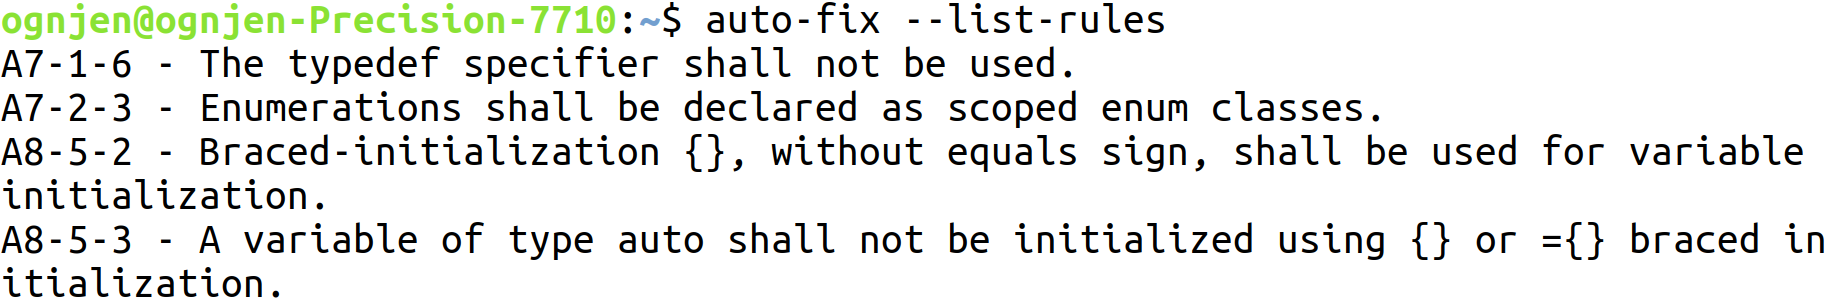
\includegraphics[scale=0.4]{listRules.png}
    \end{center}
    \caption{Ispis alata \textit{AutoFix} prilikom kori\v{s}\'{c}enja opcije \texttt{--list-rules}.}
    \label{fig:listRules}
    \end{figure}

    \item \texttt{--rules=<string>}: Ova opcija omogu\'{c}ava navođenje podskupa implementiranih pravila za koje \'{c}e alat izvr\v{s}iti analizu. Pravila u okviru ove opcije
    se navode po svojoj oznaci iz \textsc{autosar} dokumenta i treba ih razdvojiti zarezom. Ukoliko se umesto opcije pravila prosledi string \texttt{"all"} alat \'{c}e pokrenuti
    analizu sa svim implementiranim pravilima u okviru alata. Ukoliko se ova opcija ne navede prilikom pokretanja, \textit{AutoFix} \'{c}e ovo protuma\v{c}iti kao da je navedena opcija \texttt{--rules=""}, odnosno ne\'{c}e se izvr\v{s}iti analiza ni za jedno pravilo.
    Primer kori\v{s}\'{c}enja ove opcije: \newline\newline
    \texttt{auto-fix ./AutoFixTest.cpp --rules="A7\_2\_3, A7\_1\_6"} \\
    \item \texttt{--help}: Ovom opcijom se ispisuje uputstvo za upotrebu alata.
  \end{description}

Pored opcija koje su definisane u okviru alata \textit{AutoFix}, prilikom pokretanja alata mogu se dodati i opcije koje se prosleđuju kompilatoru \textit{Clang}. Na primer, mo\v{z}e da bude korisno da se navede opcija \texttt{-Wno-everything} kako bi se prijavljivala isklju\v{c}ivo upozorenja generisana alatom \textit{AutoFix} i ignorisala sva upozorenja koja generi\v{s}e kompilator \textit{Clang} tokom kompilacije. Ovo se mo\v{z}e posti\'{c}i komandom: \\ \\
\texttt{./auto-fix --rules="all" test.cpp --extra-arg="-Wno-everything" --}


\section{Opis implementiranih pravila}

Pored formalne klasifikacije opisane u sekciji \ref{sec:klasifikacija}, pravila u okviru dokumenta koji opisuje standard kodiranja \textsc{autosar} C++14 \cite{AutosarGuidelines} strukturirana su po poglavljima.
Struktura poglavlja ovog dokumenta slična je strukturi iz samog C++ standarda ISO/IEC 14882:2014. Svako poglavlje odgovara jednoj komponenti (svojstvu) jezika C++14, to jest sadrži pravila koja se odnose na tu komponentu.
\\
\indent
Pravila razmatrana u ovom radu predstavljaju podskup pravila koja se odnose na deklaracije. Deklaracije predstavljaju jedan
od osnovnih i najvažnijih koncepta u programskom jeziku C++ i programiranju generalno.
\\
\indent
Sva implementirana pravila u okviru alata \textit{AutoFix} spadaju, prema klasifikaciji iz sekcije \ref{sec:klasifikacija}, u sledeće kategorije:
\begin{enumerate}
  \item{Obavezna, prema klasifikaciji po obavezi.}
  \item{Automatizovana, prema klasifikaciji po primenjivosti statičke analize.}
  \item{Implementaciona, prema klasifikaciji po cilju primene.}
\end{enumerate}
Pravila razmatrana u okviru ovog rada birana su tako da se k\^{o}d koji nije u saglasnosti sa pravilom mo\v{z}e detektovati analizom apstraktnog sintaksi\v{c}kog stabla kompilatora \textit{Clang} i da se za taj k\^{o}d mogu kreirati razumne alternative koje su u skladu sa standardom \textsc{autosar} C++14.
Implementirana su pravila \textbf{A8-5-3}, \textbf{A8-5-2}, \textbf{A7-1-6}, \textbf{A7-2-3}.

\subsection{Pravilo A8-5-3}
\begin{center}
\begin{tcolorbox}
Promenljiva tipa \texttt{auto} ne sme biti inicijalizovana kori\v{s}\'{c}enjem viti\v{c}astih zagrada tipa \{\} ili =\{\}.
\end{tcolorbox}
\end{center}

Po standardu C++14, kompilator \'{c}e  promenljivu deklarisanu specifikatorom \texttt{auto} koja je inicijalizovana sintaksom viti\v{c}astih zagrada (\texttt{\{\}} ili \texttt{=\{\}}) tretirati kao objekat klase
\texttt{std::initializer\_list<type>}. Ukoliko programer nije svestan ove \v{c}injenice, mo\v{z}e pomisliti da \'{c}e zaklju\v{c}eni tip zapravo biti \texttt{type}. Da bi se izbegla konfuzija oko zaklju\v{c}ivanja
tipova, \textsc{autosar} standard nala\v{z}e da se ne koristi nijedna od navedene dve vrste inicijalizacije.
Na listingu \ref{lst:label13} prikazan je k\^{o}d nad kojim \'{c}e biti ilustrovana podr\v{s}ka pravilu \textbf{A8-5-3} u okviru alata \textit{AutoFix}. 
Zaklju\v{c}en tip za promenljive \texttt{x2} (linija 7) i \texttt{x4} (linija 11) bi\'c{e} \texttt{std::initializer\_list<int>}, dok \'{c}e za promenljive \texttt{x1} (linija 5) i \texttt{x3} (linija 9) biti zaklju\v{c}en tip \texttt{int}. S obzirom da deklaracije promenljivih \texttt{x2} i \texttt{x4} koriste sintaksu
viti\v{c}astih zagrada, ove deklaracije nisu napisane u skladu sa pravilom \textbf{A8-5-3}.
Na slici \ref{fig:A8-5-3} prikazan je ispis alata \textit{AutoFix} za k\^{o}d sa listinga \ref{lst:label13}. Alat u oba slu\v{c}aja predla\v{z}e
da promenljiva bude deklarisana koriste\'{c}i simbol \texttt{=}.

\begin{lstlisting}[style=customc, caption={K\^{o}d nad kojim je demonstrirana podr\v{s}ka pravilu \textbf{A8-5-3} u okviru alata \textit{AutoFix}. Ispis alata \textit{AutoFix} nakon pokretanja nad ovim kodom prikazan je na slici \ref{fig:A8-5-3}.}, label=lst:label13]
#include <initializer_list>

void fn() {
  // Compliant with rule A8-5-3.
  auto x1(10);
  // Not compliant with rule A8-5-3.
  auto x2{10};
  // Compliant with rule A8-5-3.
  auto x3 = 10;
  // Not compliant with rule A8-5-3.
  auto x4 = {10};
}

\end{lstlisting}

\begin{figure}[!h]
\begin{center}
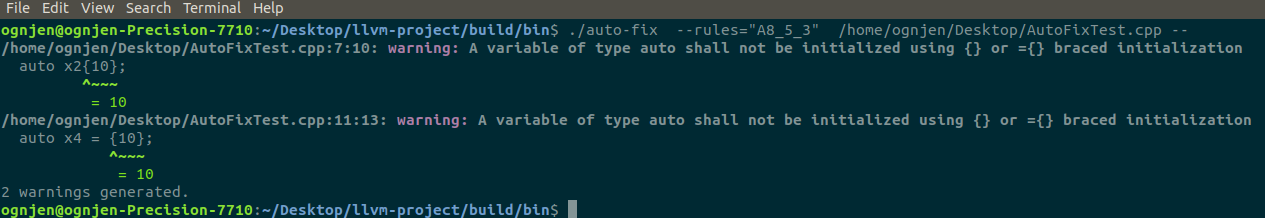
\includegraphics[scale=0.3]{A8_5_3.png}
\end{center}
\caption{Ispis alata za pravilo \textbf{A8-5-3} za k\^{o}d sa listinga \ref{lst:label13}.}
\label{fig:A8-5-3}
\end{figure}

\subsection{Pravilo A8-5-2}
\begin{center}
\begin{tcolorbox}
Inicijalizacija viti\v{c}astim zagradama bez simbola jednako (\texttt{=}) treba biti kori\v{s}\'{c}ena za inicijalizaciju promenljive.
\end{tcolorbox}
\end{center}

Po standardu C++14, prilikom upotrebe inicijalizacije viti\v{c}astih zagrada bez znaka \texttt{=} ne\'{c}e do\'{c}i do konverzija tipova iz tipa ve\'{c}e bitske \v{s}irine u tip manje bitske \v{s}irine (eng.~\textit{narrowing conversions}) \v{s}to se moze dogoditi prilikom upotrebe ostalih vrsta inicijalizacija.
Upotreba simbola \texttt{=} pri inicijalizaciji mo\v{z}e izazvati konfuziju kod programera i navesti ga na pomisao da se nad objektom poziva operator dodele iako se zapravo poziva konstruktor.
Na listingu \ref{lst:label14} prikazan je k\^{o}d nad kojim je demonstrirana podr\v{s}ka pravilu \textbf{A8-5-2} u okviru alata \textit{AutoFix}.
Deklaracije promenljivih \texttt{x1} (linija 6), \texttt{x2} (linija 8) i \texttt{x3} (linija 10) nisu u skadu sa pravilom \textbf{A8-5-2} s obzirom da ne koriste inicijalizaciju viti\v{c}astih zagrada bez simbola \texttt{=}.
Ispis alata \textit{AutoFix} kada se pokrene nad fajlom sa kodom iz listinga \ref{lst:label14} prikazan je na slici \ref{fig:A8-5-2}. \\

\begin{lstlisting}[style=customc, caption={K\^{o}d nad kojim je demonstrirana podr\v{s}ka pravilu \textbf{A8-5-2} u okviru alata \textit{AutoFix}.}, label=lst:label14]
#include <cstdint>
#include <initializer_list>

void f1() {
  // Not compliant with rule A8-5-2.
  std::int32_t x1 = 8;
  // Not compliant with rule A8-5-2.
  std::int8_t x2(x1);
  // Not compliant with rule A8-5-2.
  std::int8_t x3 = {50};
  // Compliant with rule A8-5-2.
  std::int8_t x4{50};
}
\end{lstlisting}

\begin{figure}[!h]
\begin{center}
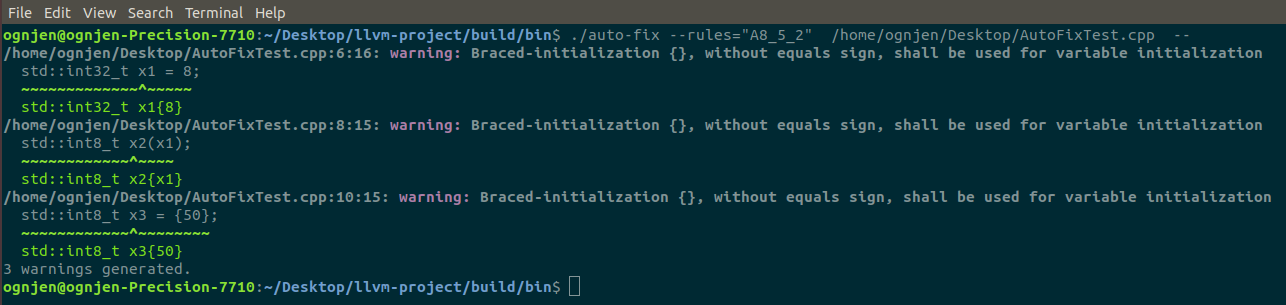
\includegraphics[scale=0.3]{A8_5_2.png}
\end{center}
\caption{Ispis alata za pravilo \textbf{A8-5-2} za k\^{o}d sa listinga \ref{lst:label14}.}
\label{fig:A8-5-2}
\end{figure}

\subsection{Pravilo A7-1-6}
\begin{center}
\begin{tcolorbox}
Ne treba koristiti specifikator \texttt{typedef}. 
\end{tcolorbox}
\end{center}

Specifikator \texttt{typedef} nije pogodan za kreiranje pseudonima (eng.~\textit{alias}) za \v{s}ablonske tipove i \v{c}ini k\^{o}d manje \v{c}itljivim.
Oba nedostatka mogu se zaobi\'{c}i kori\v{s}\'{c}enjem specifikatora \texttt{using}.  Ispis alata \textit{AutoFix} kada se pokrene nad fajlom sa kodom iz listinga \ref{lst:typedef} prikazan je na slici \ref{fig:A7-1-6}. Alat \textit{AutoFix} od izraza za kreiranje pseudonima za tip kori\v{s}\'{c}enjem
specifikatora \texttt{typedef} kreira i ispisuje analogni izraz koji koristi sintaksu sa specifikatorom \texttt{using}.

\begin{lstlisting}[style=customc, caption={Primer koda koji nije napisan u skladu sa pravilom \textbf{A7-1-6}, odnosno koristi specifikator \texttt{typedef}.}, label=lst:typedef]
#include <cstdint>

// Not compliant with rule A7-1-6.
typedef unsigned long ulong;
// Not compliant with rule A7-1-6.
typedef std::int32_t (*fPointer1)(std::int32_t);
// Not compliant with rule A7-1-6.
typedef int int_t, *intp_t;

\end{lstlisting}

\begin{figure}[!h]
\begin{center}
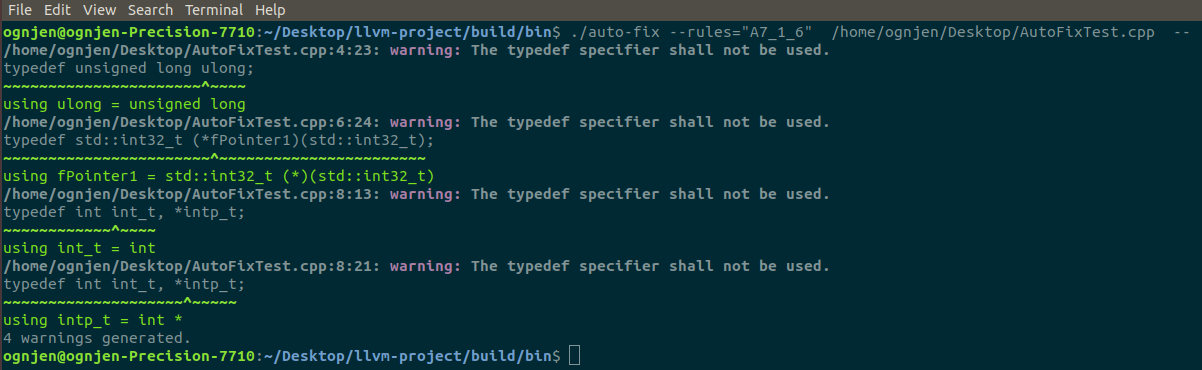
\includegraphics[scale=0.3]{A7_1_6.png}
\end{center}
\caption{Ispis alata za pravilo A7-1-6 za k\^{o}d sa listinga \ref{lst:typedef}.}
\label{fig:A7-1-6}
\end{figure}


\subsection{Pravilo A7-2-3}
\begin{center}
\begin{tcolorbox}
Nabrajanja (eng.~\textit{enumerators}) treba deklarisati kao nabrajanja sa opsegom odnosno treba koristiti sintaksu \texttt{enum class}.
\end{tcolorbox}
\end{center}

Ukoliko se prilikom deklaracije nabrajanja ne koristi sintaksa \texttt{enum class} mo\v{z}e do\'{c}i do ponovnog deklarisanja konstanti iz
globalnog opsega. Na listingu \ref{lst:redeclaration} deklarisano je nabrajanje \texttt{E1} (linija 3) koje defini\v{s}e promenljive \texttt{E10}, \texttt{E11}
i \texttt{E12} u globalnom opsegu. Ukoliko programer nije svestan \v{c}injenice da su promenljive \texttt{E10}, \texttt{E11}
i \texttt{E12} definisane u globalnom opsegu mo\v{z}e poku\v{s}ati da deklari\v{s}e globalnu promenljivu sa identifikatorom koji je kori\v{s}\'{c}en u okviru nabrajanja (linija 6). Ovo \'{c}e rezultovati gre\v{s}kom prilikom kompilacije zbog dvostruke deklaracije promenljive sa istim identifikatorom.

\begin{lstlisting}[style=customc, caption={Primer koda u okviru kog dolazi do dvostruke deklaracije promenljive sa istim identifikatorom.}, label=lst:redeclaration]
#include <cstdint>

enum E1 : std::int32_t { E10, E11, E12 };

// Compilation error. Redeclaration of E10.
static std::int32_t E10; 
\end{lstlisting}
Kori\v{s}\'{c}enjem nabrajanja sa opsegom, odnosno upotrebom sintakse \texttt{enum class}, identifikatori kori\v{s}\'{c}eni prilikom
nabrajanja bi\'{c}e deklarisani u svom unutra\v{s}njem opsegu i time spre\v{c}iti mogu\'{c}nost dvostruke deklaracije identifikatora u globalnom opsegu.

Ispis alata \textit{AutoFix} kada se pokrene nad fajlom sa kodom iz listinga \ref{lst:enum} prikazan je na slici \ref{fig:A7-2-3}. 
Alat pokazuje na koju lokaciju treba umetnuti specifikator \texttt{class}.
\\

\begin{lstlisting}[style=customc, caption={Primer koda koji nije napisan u skladu sa pravilom \textbf{A7-2-3}, odnosno ne koristi sintaksu \texttt{enum class}.}, label=lst:enum]
#include <cstdint>

// Not compliant with rule A7-2-3.
enum E1 : std::int32_t { E10, E11, E12 };

\end{lstlisting}


\begin{figure}[!h]
\begin{center}
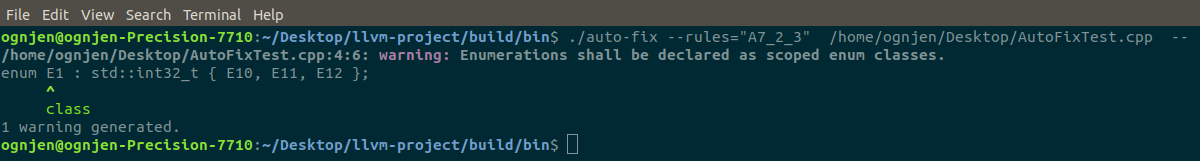
\includegraphics[scale=0.3]{A7_2_3.png}
\end{center}
\caption{Ispis alata za pravilo \textbf{A7-2-3} za k\^{o}d sa listinga \ref{lst:enum}.}
\label{fig:A7-2-3}
\end{figure}

\section{Opis implementacije alata}

Alat \textit{AutoFix} implementiran je u okviru projekta \texttt{clang-tools-extra}, potprojekta kompilatorske infrastrukture LLVM. Projekat \texttt{clang-tools-extra} sadr\v{z}i alate implementirane interfejsima za alate kompilatora \textit{Clang} (eng.~\textit{Clang’s tooling APIs}).
Alat \textit{AutoFix} je podeljen na \v{c}etiri jedinice prevođenja: \texttt{AutoFix.cpp}, \texttt{AutoFix\-Matchers.cpp}, \texttt{AutoFixDiagnosticConsumer.cpp} i \texttt{AutoFixHelper.cpp}.

\subsection{AutoFixMatchers.cpp}
Alat \textit{AutoFix} koristi biblioteku \texttt{LibAstMatchers} za analizu i obradu apstraktnog sintaksi\v{c}kog stabla kompilatora \textit{Clang}. 
\textit{AutoFix} defini\v{s}e upariva\v{c}e za uparivanje osnovnih konstrukta na koje se pravilo odnosi i za su\v{z}avanje pretrage apstraktnog sintaksi\v{c}kog stabla. Na primer, ukoliko je pravilo vezano za enumeratore (nabrajanja), upariva\v{c} koji odgovara ovom pravilu \'{c}e upariti sve deklaracije enumeratora iz apstraktnog sintaksi\v{c}kog stabla ali \'{c}e i suziti pretragu tako \v{s}to \'{c}e uparivati samo deklaracije koje nisu implicitne. Ovo se mo\v{z}e posti\'{c}i izrazom za uparivanje \texttt{enumDecl(unless(isImplicit()))}. Svakom pravilu koje alat \textit{AutoFix} podr\v{z}ava odgovara jedan upariva\v{c}. Upariva\v{c}i su nazvani po broju pravila na koje se odnose i imaju imena
\texttt{A7\_1\_6\_Matcher}, \texttt{A7\_2\_3\_Matcher}, \texttt{A8\_5\_2\_Matcher} i \texttt{A8\_5\_3\_Matcher}.
\par
 Za svaki od upariva\v{c}a implementirana je i klasa povratnog poziva u okviru koje se vr\v{s}i analiza uparenih konstrukta, konstrukcija predloga za ispravljanje koda i prijavljivanje upozorenja ukoliko je analizom utvrđeno da k\^{o}d nije napisan u skladu sa pravilom na koje se upariva\v{c} odnosi. Klase
 povratnih poziva su takođe nazvane po pravilima na koje se odnose i nose imena \texttt{A7\_1\_6}, \texttt{A7\_2\_3}, \texttt{A8\_5\_2} i \texttt{A8\_5\_3}.
\subsection{AutoFix.cpp}
Ova jedica prevođenja predstavlja ulaznu ta\v{c}ku alata \textit{AutoFix}. U okviru nje, implementirane su klase \texttt{AutoFixConsumer} i \texttt{AutoFixAction} koje nasleđuju redom klase \texttt{ASTConsumer} i \texttt{ASTFrontendAction} (opisane u sekciji \ref{sec:interfejsi}). Osnovna uloga klase \texttt{AutoFixConsumer} jeste da obezbedi da se nad jedinicom prevođenja pokrenu odgovaraju\'{c}i upariva\v{c}i. To su upariva\v{c}i koji odgovaraju pravilima koje je korisnik zadao u okviru opcije komandne linije \texttt{--rules}. Parsiranje ove opcije i  pokretanje upariva\v{c}a nad apstraktnim sintaksnim stablom implementirano je u okviru metode \texttt{HandleTranslation\-Unit} klase \texttt{AutoFixConsumer}. Ova metoda se poziva tokom parsiranja na kraju izgradnje apstraktnog sintaksi\v{c}kog stabla za svaku jedinicu prevođenja nad kojom je pokrenut alat. Klasa \texttt{AutoFixAction} instancira objekat klase \texttt{AutoFixConsumer} u okviru metode \texttt{CreateASTConsumer}.
Na slici \ref{fig:uml1} prikazan je odnos klasa \texttt{AutoFixConsumer}, \texttt{AutoFixAction}, \texttt{ASTConsumer} i \texttt{ASTFrontendAction}. \par
U okviru jedinice prevođenja \texttt{Autofix.cpp} takođe je implementirana funkcija \texttt{main} alata \textit{AutoFix}. U okviru nje vr\v{s}i se parsiranje opcija komandne linije, kreira se instanca alata, kreiranoj instanci se pridru\v{z}uje objekat klase \texttt{AutoFix\-DiagnosticConsumer} i alat se pokre\'{c}e nad zadatom jedinicom prevođenja. 

\begin{figure}
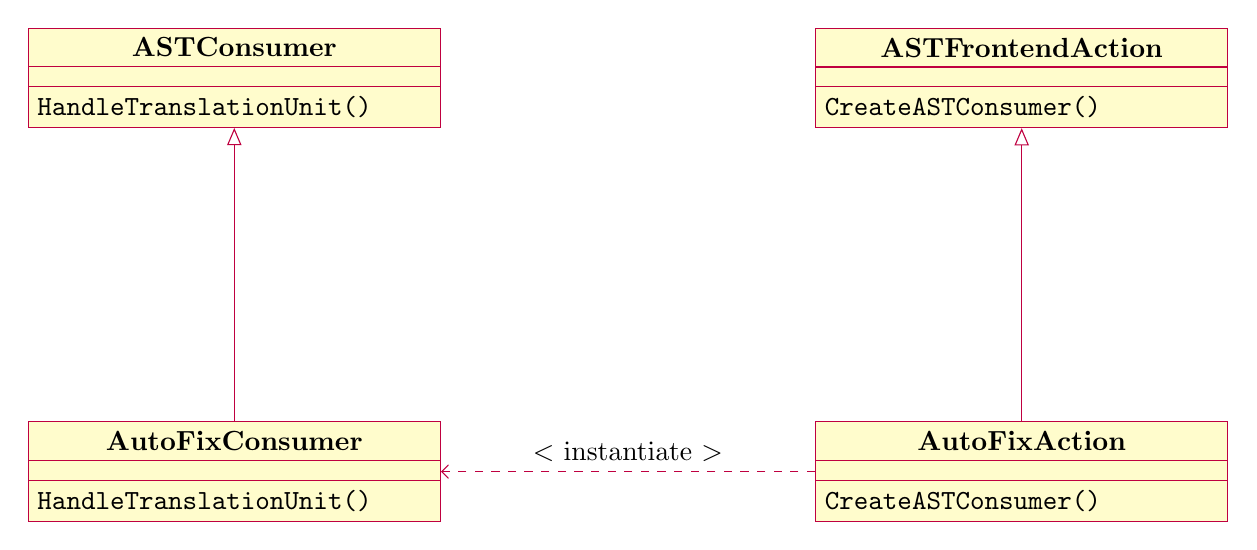
\begin{tikzpicture}
  \begin{class}[text width=5cm]{ASTConsumer}{-9, 0}
    \operation{\texttt{HandleTranslationUnit()}}
    % \operation[0]{withdrawl(amount : Dollars)}
  \end{class}
  \begin{class}[text width=5cm]{AutoFixConsumer}{-9,-5}
    \inherit{ASTConsumer}
    \operation{\texttt{HandleTranslationUnit()}}
  \end{class}

  \begin{class}[text width=5cm]{ASTFrontendAction}{1, 0}
    \operation{\texttt{CreateASTConsumer()}}
    % \operation[0]{withdrawl(amount : Dollars)}
  \end{class}
  \begin{class}[text width=5cm]{AutoFixAction}{1, -5}
    \inherit{ASTFrontendAction}
    \operation{\texttt{CreateASTConsumer()}}
  \end{class}
    \draw[umlcd style dashed line ,->] (AutoFixAction) --node[above, sloped, black]{$<$ instantiate $>$} (AutoFixConsumer) ;
\end{tikzpicture}
  \caption{Odnos klasa \texttt{ASTConsumer}, \texttt{AutoFixConsumer}, \texttt{ASTFrontendAction} i \texttt{AutoFixAction}.}
  \label{fig:uml1}

\end{figure}
\subsection{AutoFixDiagnosticConsumer.cpp}
Vid obrade dijagnostike najrelevantniji za alat \textit{AutoFix} jeste njeno ispisivanje na standardni izlaz. U ovu 
svrhu \textit{AutoFix} koristi funkcionalnost postoje\'{c}e klase \texttt{TextDiagnosticPrinter} (opisane u sekciji \ref{sec:diagnostics}).
Pored ispisivanja poruka upozorenja i predloga za ispravljanje koda na standardni izlaz, alat \textit{AutoFix} konzumira dijagnostiku tako \v{s}to predlo\v{z}ene izmene koda primenjuje na izvorni fajl ukoliko je prosleđena opcija komandne linije \texttt{--apply-fix}.
Da bi se ovo postiglo u okviru alata \textit{AutoFix} implementirana je klasa \texttt{AutoFix\-DiagnosticConsumer}. Ova klasa nasleđuje
klasu \texttt{TextDiagnosticPrinter} i time zadr\v{z}ava funkcionalnost ispisivanja dijagnostike na standardni izlaz koja je implementirana u okviru nje. \par Klasa \texttt{AutoFixDiagnosticConsumer} predefini\v{s}e metod \texttt{HandleDiag\-nostic} i u okviru njega pored ispisivanja dijagnostike kreira objekat klase \texttt{Replace\-ment} za predlo\v{z}enu izmenu koda. Objekat klase \texttt{Replacement} \v{c}uva putanju do fajla (\texttt{std::\-string FilePath}), informacije o tome koje delove izvornog koda treba zameniti sa predlogom za ispravljanje koda i sam predlog (\texttt{Range ReplacementRange}, \texttt{std::string ReplacementText}).
U okviru metode \texttt{finish} svi kreirani objekti klase \texttt{Replacement} se pridru\v{z}uju objektu klase \texttt{Rewriter}.
Ova klasa omogu\'{c}ava primenjivanje predlo\v{z}enih izmena koda na izvorni fajl. Predlo\v{z}ene izmene koda primenjuju se pozivom metode \texttt{overwriteChangedFiles} klase \texttt{Rewriter}. Na slici \ref{fig:DiagnosticConsumer} prikazan je odnos klasa \texttt{DiagnosticConsumer}, \texttt{TextDiagnosticPrinter}, \texttt{AutoFixDiagnosticConsumer}, \texttt{Rewriter} i \texttt{Replacement}.

\begin{center}
\begin{figure}
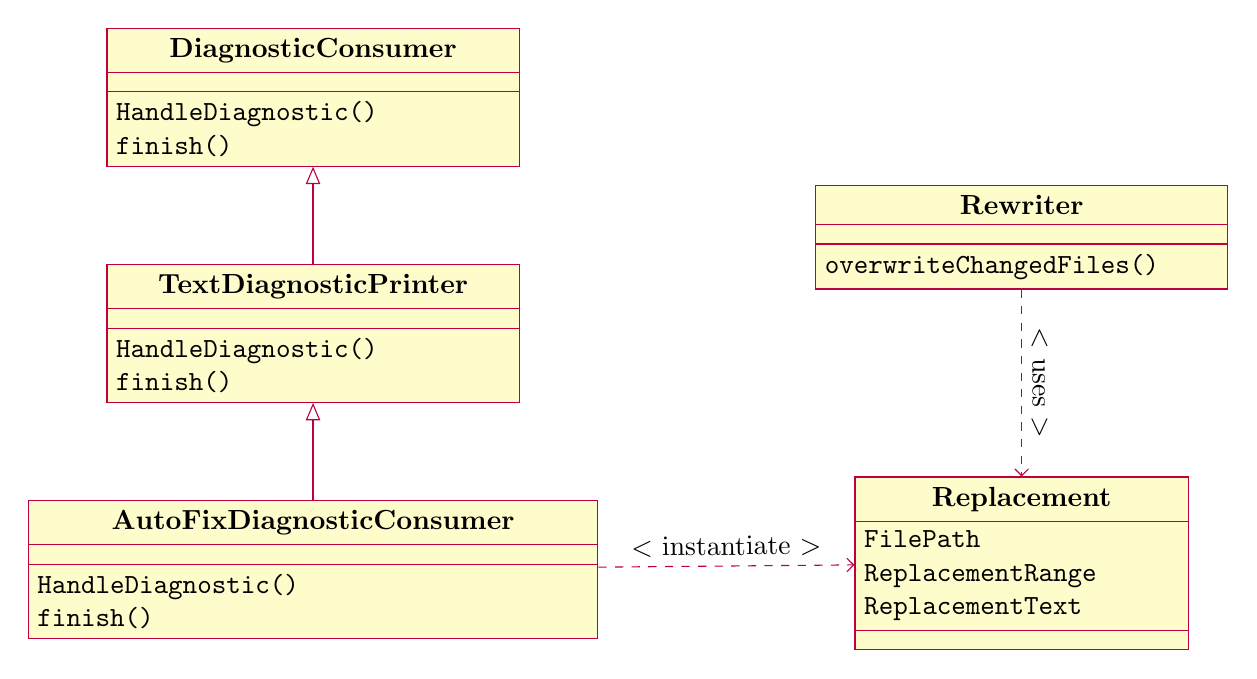
\begin{tikzpicture}
  \begin{class}[text width=5cm]{DiagnosticConsumer}{-9, 0}
    \operation{\texttt{HandleDiagnostic()}}
    \operation{\texttt{finish()}}
  \end{class}
  \begin{class}[text width=5cm]{TextDiagnosticPrinter}{-9, -3}
    \inherit{DiagnosticConsumer}
    \operation{\texttt{HandleDiagnostic()}}
    \operation{\texttt{finish()}}
  \end{class}

  \begin{class}[text width=7cm]{AutoFixDiagnosticConsumer}{-9, -6}
    \inherit{TextDiagnosticPrinter}
    \operation{\texttt{HandleDiagnostic()}}
    \operation{\texttt{finish()}}
  \end{class}
  \begin{class}[text width=4cm]{Replacement}{0, -5.7}
  \attribute{\texttt{FilePath}}
  \attribute{\texttt{ReplacementRange}}
  \attribute{\texttt{ReplacementText}}
  \end{class}
  \begin{class}[text width=5cm]{Rewriter}{0, -2}
  \operation{\texttt{overwriteChangedFiles()}}
  \end{class}
    \draw[umlcd style dashed line ,->] (AutoFixDiagnosticConsumer) --node[above, sloped, black]{$<$ instantiate $>$} (Replacement) ;
    \draw[umlcd style dashed line ,->] (Rewriter) --node[above, sloped, black]{$<$ uses $>$} (Replacement) ;

\end{tikzpicture}
  \caption{Odnos klasa \texttt{DiagnosticConsumer}, \texttt{TextDiagnosticPrinter}, \texttt{AutoFixDiagnosticConsumer}, \texttt{Rewriter} i \texttt{Replacement}.}
  \label{fig:DiagnosticConsumer}

\end{figure}
\end{center}

\subsection{AutoFixHelper.cpp}

U okviru jedinice prevođenja \texttt{AutoFixHelper.cpp} implementirane su pomo\'{c}ne funkcije kori\v{s}\'{c}ene u okviru alata \textit{AutoFix}. U nastavku su ukratko opisane funkcije iz ove jedinice prevođenja.
\begin{itemize}
  \item \texttt{getWordsFromString} --- kreira niz re\v{c}i od stringa prosleđenog u okviru opcija komandne linije.
  \item \texttt{getExprStr} --- kreira string od \v{c}vorova apstraktnog sintaksi\v{c}kog stabla tipa \texttt{Expr}.
  \item \texttt{getChildOfType} - pronalazi dete \v{c}vora iz apstraktnog sintaksi\v{c}kog stabla koje ima određeni tip.
  \item \texttt{trimString} --- Izbacuje prazne karaktere (eng.~\textit{whitespace characters}) sa po\v{c}etka i sa kraja stringa.
  \item \texttt{trimBraces} --- Izbacuje karakter \texttt{\{} sa po\v{c}etka i karakter \texttt{\}} sa kraja stringa.
\end{itemize}

\section{Opis testiranja alata}

U okviru alata \textit{AutoFix} testirana je implementacija svakog od podr\v{z}anih pravila. Svaki test proverava implementaciju jednog pravila.
Testovi \texttt{auto-fix-A7-1-6\-.cpp}, \texttt{auto-fix-A7-2-3.cpp}, \texttt{auto-fix-A8-5-2.cpp} i \texttt{auto-fix-A8-5-3.cpp} nalaze se u okviru direktorijuma \texttt{autofix-test} i redom testiraju implementaciju pravila
\textbf{A7-1-6}, \textbf{A7-2-3}, \textbf{A8-5-2} i \textbf{A8-5-3}. C++ k\^{o}d u okviru testova, nad kojim je testirana ispravnost rada alata, ve\'c{i}nski je preuzet iz primera u okviru dokumenta u kom je opisan standard \textsc{autosar} C++14 \cite{AutosarGuidelines}. Testovi su dopunjeni kodom za koji je autor ovog rada smatrao da ilustruje bitne  slu\v{c}ajeve upotrebe a ne nalazi se u okviru primera iz dokumenta.

Na listingu \ref{lst:test} prikazan je pojednostavljeni primer testa za pravilo \textbf{A7-1-6} u okviru alata \textit{AutoFix}. Test je pojednostavljen tako \v{s}to se u okviru njega nalazi samo jedan konstrukt koji nije u skladu sa pravilom \textbf{A7-1-6}. Pojednostavljeni test je kori\v{s}\'{c}en kako bi se demonstrirali svi bitni aspekata testiranja alata \textit{AutoFix} sa \v{s}to manje koda. \par Test
proverava da se pokretanjem alata \texttt{AutoFix} ispisuje adekvatno upozorenje zajedno sa predlogom za ispravljanje koda. U okviru \texttt{RUN} linije (linija 1) pokre\'{c}e se alat \textit{AutoFix} komandom \texttt{auto-fix --rules="A7\_1\_6" \%s 2>\&1 --}. Simbol \texttt{\%s}  \'{c}e prilikom pokretanja biti zamenjen putanjom do testa u kome se ova komanda nalazi (testa koji \textit{lit} pokre\'{c}e). \texttt{2>\&1} preusmerava standardni izlaz za gre\v{s}ke (STDERR) na standardni izlaz (STDOUT). Drugi deo komande \texttt{| FileCheck \%s} prosleđuje izlaz iz alata \textit{AutoFix} na standardni ulaz alata \textit{FileCheck} i pokre\'{c}e alat \textit{FileCheck} nad testom. Putanja do testa prosleđena je simbolom \texttt{\%s} \cite{LIT}.

 U okviru listinga \ref{lst:test} koriste se tri direktive alata \textit{FileCheck}, \texttt{CHECK: TEKST} (linija 6), \texttt{CHECK-NEXT: TEKST} (linije 8-11) i \texttt{CHECK-NOT: TEKST} (linije 5 i 12). Ove direktive slu\v{z}e da se izvr\v{s}i provera da li je alat ispisao upozorenje vezano za pravilo \textbf{A7-1-6}, predlog za ispravljanje koda i da se u okviru ispisa nije na\v{s}lo nijedno drugo upozorenje. U okviru direktive \texttt{CHECK} koriste se regularni izrazi za putanju na operativnom sistemu Linuks (eng.~\textit{Linux}), za po\v{c}etak i kraj linije. Redom, ovo su regularni izrazi \lstinline[style=custombash]{(/|/[a-zA-Z0-9_-]+)+}, \lstinline[style=custombash]{^} i \lstinline[style=custombash]{$}. Upotrebom regularnih izraza za po\v{c}etak i kraj linije test proverava da alat \textit{AutoFix} nije ispisao ni\v{s}ta nepredviđeno, odnosno da svaka linija po\v{c}inje i zavr\v{s}ava se tekstom navedenim između ta dva regularna izraza. Regualrni izraz za putanju na operativnom sistemu Linux koristi se kako test ne bi o\v{c}ekivao specifi\v{c}nu apsolutnu putanju u okviru ispisa alata \textit{AutoFix}. 

\begin{lstlisting}[style=customc, caption={Pojednostavljeni primer testa za pravilo \textbf{A7-1-6} u okviru alata \textit{AutoFix}.},label={lst:test}]
// RUN: auto-fix --rules="A7_1_6" %s 2>&1 -- | FileCheck %s

typedef unsigned long ulong;

// CHECK-NOT: {{.+}}
// CHECK: {{^((/|/[a-zA-Z0-9_-]+)+)}}/auto-fix-A7-1-6.cpp:3:23: warning: The typedef specifier shall not be used.{{$}}
// CHECK-NEXT: {{^}}typedef unsigned long ulong;{{$}}
// CHECK-NEXT: {{^}}~~~~~~~~~~~~~~~~~~~~~~^~~~~{{$}}
// CHECK-NEXT: {{^}}using ulong = unsigned long{{$}}
// CHECK-NEXT: {{^}}1 warning generated.{{$}}
// CHECK-NOT: {{.+}}
\end{lstlisting}

\section{Analiza rezultata rada alata}

U svrhu provere robusnosti i kvaliteta alata \textit{AutoFix}, izvr\v{s}ena je analiza nad delovima projekta \textit{Automotive Grade Linux (AGL)} \cite{AGL}. Projekat \textit{AGL} je izabran na osnovu svoje relevantnosti u automobilskoj industriji. \par

\textit{AGL} je zajedni\v{c}ki projekat otvorenog koda koji okuplja proizvođa\v{c}e automobila, dobavlja\v{c}e i tehnolo\v{s}ke kompanije kako bi ubrzao razvoj i usvajanje potpuno otvorenog softverskog paketa (eng.~\textit{software stack}) za povezane automobile (eng.~\textit{connected cars}). Sa operativnim sistemom Linuks u svojoj osnovi, AGL razvija platformu koja mo\v{z}e slu\v{z}iti kao \textit{de facto} standard u industriji \v{c}ime bi se omogu\'{c}io brz razvoj novih funkcija i tehnologija \cite{AGL}.
\par
Alat \textit{AutoFix} pokretan je nad dva podprojekta projekta \textit{AGL}. To su projekti \textit{re2c} i \textit{ninja}. Projekti su izabrani nasumi\v{c}no osim kriterijuma
da opseg projekta bude relativno mali. Analiza rezultata rada alata, odnosno upozorenja koje je alat \textit{AutoFix} prijavio, izvr\v{s}ena je ru\v{c}no od strane autora ovog rada. Kriterijum da projekat bude manjeg obima kori\v{s}\'{c}en je kako bi se smanjila verovatno\'{c}a gre\v{s}ke prilikom pomenute analize rezultata. Alat je pokretan skriptom koji rekurzivno 
obilazi direktorijume u okviru projekta i pokre\'{c}e alat \textit{AutoFix} nad  svim fajlovima sa ekstenzijom \texttt{.cpp} i \texttt{.cc}. Nad svakim fajlom, alat je pokrenut komandom \\
\texttt{./auto-fix  --rules="all"  putanja\_do\_fajla }

\subsection{Projekat \textit{re2c}}

Projekat \textit{re2c} nad kojim je pokretan alat \textit{AutoFix} nalazi se u okviru projekta \textit{AGL} na lokaciji \texttt{build/tmp/work/x86\_64-linux/re2c-native}. Projekat sadr\v{z}i 79 fajlova sa ekstenzom \texttt{.cc} \v{c}iji ukupan broj linija koda iznosi 21021. U okviru projekta
nalazi se 77 zaglavlja \v{c}iji ukupan broj linija koda iznosi 3910 \footnote{Broj linija koda je prebrojan alatom \textit{cloc}. Alat je dostupan na linku \url{http://cloc.sourceforge.net/}.}. \par
Tabela \ref{fig:re2c} prikazuje broj prijavljenih upozorenja za svako od pravila prilikom pokretanja alata \textit{AutoFix}.
Za svako od upozorenja ispisan je i odgovaraju\'{c}i predlog za ispravljanje koda. Upozorenje za pravilo \textbf{A8-5-3} nije prijavljeno nijednom. Pretragom
alatom \textit{grep} kroz svaki od fajlova ustanovljeno je da konstrukti na koje se odnosi pravilo \textbf{A8-5-3} zaista nisu kori\v{s}\'{c}eni u okviru koda i da se ne radi o gre\v{s}ci u alatu \textit{AutoFix}. Ovaj rezultat sla\v{z}e se sa \v{c}injenicom da je najve\'{c}i broj upozorenja prijavljen za pravilo \textbf{A8-5-2}. Pravilo \textbf{A8-5-2} predla\v{z}e upotrebu inicijalizacije viti\v{c}astim zagradama pri inicijalizaciji promenljive dok pravilo \textbf{A8-5-3} zabranjuje upotrebu inicijalizacije viti\v{c}astim zagradama prilikom deklaracije promenljivih sa tipom \texttt{auto}. S obzirom na veliki broj upozorenja za pravilo \textbf{A8-5-2} i \v{c}injenice da za pravilo \textbf{A8-5-3} nije prijavljeno nijedno upozorenje, zaklju\v{c}eno je da prilikom inicijalizacije promenljivih nije kori\v{s}\'{c}ena sintaksa viti\v{c}astih zagrada ne vezano da li je promenljiva
tipa \texttt{auto} ili ne. U kombinaciji sa \v{c}injenicom da je prijavljen veliki broj upozorenja za pravila \textbf{A7-1-6} i \textbf{A8-5-2} zaklju\v{c}eno je da k\^{o}d u okviru projekta \textit{re2c} nije pisan po standardu \textsc{autosar} C++14. \par
Skript za pokretanje alata \textit{AutoFix} nad projektom \textit{re2c} pokrenut je deset puta kako bi se izra\v{c}unalo prose\v{c}no vreme izvr\v{s}avanja alata, koje iznosi 39.602 sekunde. Vreme je izmereno programom \texttt{time} u okviru operativnog sistema Linux. Izra\v{c}unato prose\v{c}no vreme se odnosi na komponentu \texttt{real} u okviru rezultata programa \texttt{time}.
\begin{table}[!h]
\begin{center}
\begin{tabular}{ |p{3cm}||p{2cm}|p{2cm}|p{2cm}|p{2cm}|  }
 \hline
 \multicolumn{5}{|c|}{Broj prijavljenih upozorenja po pravilu} \\
 \hline
 Ime projekta & Pravilo A7-1-6 & Pravilo A7-2-3 & Pravilo A8-5-2 & Pravilo A8-5-3\\
 \hline
 \textit{re2c}   & 1329            & 714             & 2561            & 0\\
 \hline
\end{tabular}
\caption{Broj prijavljenih upozorenja po pravilu za projekat \textit{re2c}.}
\label{fig:re2c}
\end{center}
\end{table}

\subsection{Projekat \textit{ninja}}

Projekat \textit{ninja} nad kojim je pokretan alat \textit{AutoFix} nalazi se u okviru projekta \textit{AGL} na lokaciji \texttt{build/tmp/work/x86\_64-linux/ninja-native}. Projekat sadr\v{z}i 55 fajlova sa ekstenzom \texttt{.cc} \v{c}iji ukupan broj linija koda iznosi 12587. U okviru projekta
nalazi se 43 zaglavlja \v{c}iji ukupan broj linija koda iznosi 2291. \par
Tabela \ref{fig:ninja} prikazuje broj prijavljenih upozorenja za svako od pravila prilikom pokretanja alata \textit{AutoFix}.
Na osnovu rezultata sa slike prime\'{c}eno je da je odnos broja prijavljenih upozorenja po pravilu sli\v{c}an rezultatima prikazanim na tabeli \ref{fig:re2c} dobijenim pri pokretanju alata \textit{AutoFix} nad projektom \textit{re2c}. Na osnovu ovoga, zaklju\v{c}ci izvedeni tokom diskusije rezultata nad projektom \textit{re2c} va\v{z}e i za rezultate projekta \textit{ninja}. Skript za pokretanje alata \textit{AutoFix} nad projektom \textit{ninja} pokrenut je deset puta kako bi se izra\v{c}unalo prose\v{c}no vreme izvr\v{s}avanja alata, koje iznosi 18.002 sekunde.\par
\begin{table}[!h]
\begin{center}
\begin{tabular}{ |p{3cm}||p{2cm}|p{2cm}|p{2cm}|p{2cm}|  }
 \hline
 \multicolumn{5}{|c|}{Broj prijavljenih upozorenja po pravilu} \\
 \hline
 Ime projekta & Pravilo A7-1-6 & Pravilo A7-2-3 & Pravilo A8-5-2 & Pravilo A8-5-3\\
 \hline
 \textit{ninja}   & 334            & 188             & 1007            & 0\\
 \hline
\end{tabular}
\caption{Broj prijavljenih upozorenja po pravilu za projekat \textit{ninja}.}
\label{fig:ninja}
\end{center}
\end{table}

\subsection{Rezime analize rezultata rada alata}
Alat se uspe\v{s}no izvr\v{s}io prilikom pokretanja nad svakim fajlom sa ekstenzijom \texttt{.cc} u okviru projekata \textit{re2c} i \textit{ninja}. Prilikom ru\v{c}ne analize upozorenja koje je alat \textit{AutoFix} prijavio nisu uo\v{c}ene gre\v{s}ke u radu alata. Na osnovu dobijenih rezultata mo\v{z}e se zaklju\v{c}iti da je alat \textit{AutoFix} robustan i da se mo\v{z}e efikasno koristiti nad realnim industrijskim projektima.



% ------------------------------------------------------------------------------

% \pangrami

% \pangrami

% ------------------------------------------------------------------------------
\chapter{Zaključak}
% ------------------------------------------------------------------------------

Standardi za pravilno pisanje koda u programskom jeziku defini\v{s}u niz pravila koje programer treba da sledi tokom razvoja softvera. Primena ovakvih standarda
tokom razvoja softvera pove\'{c}ava kvalitet softvera time \v{s}to smanjuje verovatno\'{c}u pojavljivanja gre\v{s}ke u kodu. U automobilskoj industriji,
najzastupljeniji standard za pravilno pisanje koda u jeziku C++14 je standard \textsc{autosar} C++14.
\par
Ru\v{c}no proveravanje da li je k\^{o}d napisan u skladu sa standardom predstavlja mukotrpan i neefikasan proces. U svrhu automatizovanja ovog procesa
koriste se alati za stati\v{c}ku analizu koda, koji bez pokretanja programa detektuju k\^{o}d koji nije napisan u skladu sa standardom. Alat \textit{AutoFix}, koji je razvijen u ovom radu, ispisuje upozorenja vezana za k\^{o}d koji nije napisan u skladu sa podskupom pravila iz standarda \textsc{autosar} C++14 koja se odnose na deklaracije u programskom jeziku C++14 i predla\v{z}e kako izmeniti k\^{o}d da bi bio u skladu sa standardom. \textit{AutoFix} podr\v{z}ava i opciju komandne linije kojom se predlo\v{z}ene izmene mogu primeniti na izvorni k\^{o}d. Alat je razvijen kori\v{s}\'{c}enjem biblioteka koje pru\v{z}a kompilatorska infrastruktura LLVM. Pravila standarda \textsc{autosar} C++14 podr\v{z}ana u okviru alata \textit{AutoFix} su \textbf{A8-5-3}, \textbf{A8-5-2}, \textbf{A7-1-6}, \textbf{A7-2-3}. Detaljnim testiranjem upotrebom alata \textit{lit} i \textit{FileCheck} iz kompilatorske infrastrukture LLVM obezbeđen je i visok kvalitet razvijenog alata. Analizom rezultata dobijenim pokretanjem alata \textit{AutoFix} nad podprojektima projekta \textit{AGL} zaklju\v{c}eno je da u okviru podprojekta \textit{re2c} i \textit{ninja} k\^{o}d nije napisan po standardu \textsc{autosar} C++14.

\par
U daljem razvoju alat se mo\v{z}e unaprediti na nekoliko na\v{c}ina. 
Stati\v{c}ka analiza u okviru alata mogla bi se unaprediti upotrebom naprednijih tehnika kao \v{s}to je simboli\v{c}ko izvr\v{s}avanje programa. Ovakva analiza
omogu\'{c}ila bi i podr\v{s}ku zna\v{c}ajno \v{s}ireg skupa pravila. U ovu svrhu u okviru alata \textit{AutoFix} mogao bi se integrisati stati\v{c}ki analizator kompilatora \textit{Clang} koji omogu\'{c}ava ovakav tip analize. Alat bi se mogao unaprediti i implementiranjem dodatnih opcija komandne linije koje bi omogu\'{c}ile korisniku ve\'{c}u
kontrolu nad samim alatom. Na primer, mogla bi se dodati opcija koja omogu\'{c}ava korisniku da isklju\v{c}i analizu u zadatim delovima koda.

% ------------------------------------------------------------------------------
% Literatura
% ------------------------------------------------------------------------------
\literatura

% ==============================================================================
% Završni deo teze i prilozi
\backmatter
% ==============================================================================

% ------------------------------------------------------------------------------
% Biografija kandidata
\begin{biografija}
  \textbf{Ognjen Plavšić} rođen je 14.06.1995. u Leskovcu. Zavr\v{s}io je Gimnaziju u Leskovcu, Matemati\v{c}ki smer, 2014. godine
  i iste godine upisao Matemati\v{c}ki fakultet u Beogradu. 2019. godine je zavr\v{s}io osnovne studije Matemati\v{c}kog fakulteta sa prose\v{c}nom ocenom 9.14 i iste
  godine upisao master studije. Marta 2019. godine kre\'{c}e na praksu u Nau\v{c}no-istra\v{z}iva\v{c}kom centru RT-RK (kasnije Syrmia), gde
  se oktobra iste godine zapo\v{s}ljava na poziciji softverskog in\v{z}enjera. Radio je na projektu \v{c}iji je cilj bio kreiranje alata za stati\v{c}ku analizu u okviru kompilatorske infrastrukture
  LLVM. Jula 2021. godine prelazi u kompaniju HTEC Group gde i danas
  radi kao softverski in\v{z}enjer. Trenutno se bavi kompilatorima za ma\v{s}insko u\v{c}enje
  (eng.~\textit{machine learning (ML) compilers}). U okviru ovih kompilatora radi na generisanju i optimizaciji koda od modela ma\v{s}inskog u\v{c}enja predstavljenim u nekom od formata poznatih okru\v{z}enja ma\v{s}inskog u\v{c}enja (eng.~\textit{machine learning frameworks}). Vezano za temu master teze, ima objavljen rad na međunarodnoj konferenciji \textit{ZINC} \cite{AutoCheck}: \par
  \begin{enumerate}
    \item{\textit{Milena Vujo\v{s}evi\'{c} Jani\v{c}i\'{c}, Ognjen Plav\v{s}i\'{c}, Mirko Brku\v{s}anin, Petar Jovanovi\'{c}: AUTOCHECK: A Tool For Checking Compliance With Automotive Coding Standards, 2021 Zooming Innovation in Consumer Electronics International Conference (ZINC), (Novi Sad, Serbia)}
    }
    
  \end{enumerate}

\end{biografija}
% ------------------------------------------------------------------------------

\end{document}
